\documentclass[letterpaper,11pt]{article}
\usepackage{mystyle}

% Uncomment this section if you wish to have a header.
%\usepackage{fancyhdr} 
%\pagestyle{fancy} 
%\renewcommand{\headrulewidth}{0.5pt} % customise the layout... 
%\lhead{} \chead{<++>} \rhead{<++>} 
%\lfoot{} \cfoot{\thepage} \rfoot{}


\begin{document}
\title{A Graph Parallel Implementation of Hidden Markov Models}
\author{Kevin Schmid, Andy Shi, Ding Zhou \\ CS 205 \\
Harvard College \\ Cambridge, MA}
\date{May 11, 2015}
\maketitle

% No indentation for new paragraphs
%\setlength\parindent{0pt}

% Skip a line between paragraphs
%\setlength\parskip{2ex}

% Put your stuff here

\begin{multicols*}{2}

\section{Introduction}

Hidden Markov models (HMM) are often used to model time-series data for both
discrete and continuous data. HMM has been successfully applied to problems such as speech recognition \cite{hmm-speech} and gesture recognition \cite{hmm-gesture}. The
parameters to a hidden Markov models are most commonly learned from the
Baum-Welch---an Expectation Maximization (EM) algorithm. Unfortunately, the
Baum-Welch algorithm is quadratic in number of states. A parallel implementation
of the EM algorithm along the state axis would greatly improve scalability.
Graph based platforms are particularly suited to EM algorithms, and our project
uses GraphLab~\cite{graphlab}, a platform created by Dato~\cite{dato} for implementing graph based parallelizing schemes. 

Our code is available at
\url{https://github.com/cs205-project-group/hmm}.


\section{Background}

\subsection{Hidden Markov Model}
A hidden Markov model assumes that the system follows a Markov process. For this paper, we will assume a finite number of states and observations. The probability of transitioning from state $i$ to state $j$ only depends on the current state, and we define transition matrix $A$ such that element $a_{ij}$ is the probability  of transitioning from $i$ to $j$. In an HMM, we cannot observe states, but we can observe outputs generated by the states. Given $N$ states and $M$ observations, we capture this with a $N \times M$ emission matrix $B$, where $b_{ij}$ is the probability of observation $j$ given the state is $i$. Finally, we define a $N$ length vector as $\pi$ as the prior, where $\pi_i$ is the probability of initial state being $i$. 

We can thus capture all the information about an HMM with $\theta = (A, B, \pi)$. In an HMM, we are given a sequence of $T$ observations, and we will use a series of forward and backwards propagations to estimate the parameters $\theta = (A, B, \pi)$.

\subsection{Baum-Welch}

The following explanation is based on Wikipedia's presentation of the algorithm. \cite{bwwiki}

Let $(X_1, X_2, \ldots, X_N)$ denote the $N$ states and $\bold{O} = \{O_1, O_2, \ldots, O_T\}$ the $T$ observed outputs. The Baum-Welch algorithm uses expectation-maximization to find the maximum likelihood estimate.

Suppose we begin with some initial parameters, $\theta  =  (A, B, \pi)$.  Given the observation sequence, our task is to update these parameters based on insights from the training sequence.  

Given our training sequence, Baum-Welch first figures out the probability of being in a state at some time in the ``run" of the observation sequence.  Let's call this $\gamma_{i}(t)$, the ``probability of being in state $i$ at time $t$ of this observation sequence given our current model parameters," $P(X_t = i | \bold{O}, \theta)$.

How can we figure this out? To do this, the Baum-Welch algorithm performs two sub-calculations, for the ``forward probabilities" and the ``backward probabilities."  Like $\gamma_i(t)$ values, the forward probability are computed for each ($\textit{state}, \textit{time}$) pair: given some observation sequence and our current moel, the forward probability $\alpha_i(t)$ is the probability of seeing the observation sequence up to time $t$ and landing in state $i$.  The backward probability is defined analogously: it's the probability of starting in some state $i$ and seeing the observation sequence \textit{from} time $t$ until the end.

We can define the forward and backward probabilities recursively:

\begin{equation} \label{alpha}
\alpha_i(t+1) =  b_{jo_1}\sum_{i=1}^{N} \alpha_i(t)a_{ij}
\end{equation}

\begin{equation} \label{beta}
\beta_i(t) = \sum_{i=1}^N \beta_j(t+1)a_{ij}b_j(o_{t+1})
\end{equation}

We can put the alpha and beta probabilities together to find $\gamma_i(t)$.  Some intuition for this formula: the bottom is the probability of being in \textit{some state} at time $t$ given our \textit{entire} observation sequence.  The top is the probability of being in some particular state $i$ at time $t$ given our \textit{entire} observation sequence.  For both numerator and denominator, you have to get to the state at that time (forward probability) and leave from the state next and finish emitting the observation sequence  (backward probability).

\begin{equation} \label{gamma}
\gamma_i(t) = P(X_t = i | \bold{O}, \theta) = \frac{\alpha_i(t) \beta_i(t)}{\sum_{j=1}^N \alpha_j(t) \beta_j(t)}
\end{equation}

From here, we can figure out our updates for the $B$ matrix and the new prior. 

$B$ can be updated by: 
\begin{equation}\label{b}
b^*_{i,v_k} = \frac{\sum_{t=1}^{T}1_{o_t = v_k} \gamma_i(t)}{\sum_{t=1}^T \gamma_i(t)}
\end{equation}
where $1_{o_t = v_k}$ is $1$ if $o_t = v_k$ and $0$ otherwise. 

Intuition: the update for  $b^*_{i,v_k}$ is just the frequency across the entire observation sequence of being in the state $i$ and seeing $v_k$.

\begin{equation}\label{pi}
\pi_i^* = \gamma_i(0)
\end{equation}

Intuition: this is the probability of being in state $i$ before the observation sequence begins.  

To update the $A$ matrix (each $a_{ij}$ entry), we need to figure  out the probability of being in state $i$ and $\textit{moving}$ to state $j$ next.  Fortunately, this calculation can be done in a straightforward way, and we can think of it as a ``relative frequency calculation" of the transitions that begin at state $i$ and go to state $j$ compared to the transitions through state $i$.  This ``relative frequency intuition" is provided by \cite{rabiner1986introduction}.

Define $\xi_{ij}(t)$ to be the probability of being in state $i$ at time $t$ and state $j$ at time $t+1$ given $\bold{O}$ and parameter $\theta$. 
\begin{equation}\label{xi}
\begin{aligned}
\xi_{ij}(t) &= P(X_t = i, X_{t+1} = j | \bold{O}, \theta)  \\
&=\frac{\alpha_i(t) a_{ij} \beta_j(t+1)b_{jo_{t+1}}}{\sum_{k=1}^N \alpha_k(t) \beta_k(t)}
\end{aligned}
\end{equation}
Finally, $A$ can be updated by: 

\begin{equation}\label{a}
a^*_{ij} = \frac{\sum_{t=1}^{T-1}\xi_{ij}(t)}{\sum_{t=1}^{T-1}\gamma_i(t)}
\end{equation}

These steps are repeated until the parameters converge. 

\subsection{Prior Work}

Here we review prior work related to \textit{parallelization} of hidden Markov models specifically.  In 2009, Chuan Liu conducted an independent project aiming to implement HMM training in parallel on CUDA.  The project's parallelization of the  forward-backward probabilities computation informed how we could approach parallelizing this part, even though our representation in our framework ended up distinctively graph-based.  The rest of his work frames computations in terms of matrix multiplication operations.  His work also utilizes ``parallel reduction" for computing the sum of a vector, something we've seen in CS205.  \cite{cuda-hmm}

Also, we noted the approach of Li et. al in 2010, applying an earlier parallelization approach - ``cut and stitch" - to the problem of hidden Markov model training.  The ``cut and stitch" approach parallelizes along the length of the input observation sequence (along the $T$-axis).  The graph parallel scheme in this paper is orthogonal to the ``cut and stitch" approach, and we are excited about the prospect of applying these two parallelization schemes to the problem of HMM training. \cite{cut-stitch}

\section{Approach and Secret Weapon}

\subsection{Serial Implementation}
We first implemented Baum-Welch in Python with numpy, using a mix of vectorized and non-vectorized code.  \footnote{We also used the range function instead of the xrange function in some places.  Our Python implementation also uses the default data type of numpy/Python; our later parallel implementation uses a mix of doubles and floats.  Our project desires to make a comparison based on scaling, so we don't consider these ``constant factor" sorts of differences to be an issue.}  Our initial
implementation ran into serious underflow issues from the calculations of
$\alpha$'s and $\beta$'s due to multiplying probabilities together. We solve
this by following the methods detailed by Zhai~\cite{normalizer}. We normalize by scaling $\alpha_i(t)$'s such that they sum up to $1$ over $i$'s---that is over all states. So 

\begin{equation} 
\sum_{i=1}^N \hat{\alpha}_t(i) = 1
\end{equation}

and we want to define the normalizers $\eta_k$ such that

\begin{equation} 
    \hat{\alpha}_t(i) = \alpha_i(t) \prod_{k=1}^t \frac{1}{\eta_k}
\end{equation}

then 
\begin{equation}
\prod_{k=1}^t \eta_k =\sum_{i=1}^N \alpha_t(i)
\end{equation}

We can define 
\begin{equation} 
    \hat{\beta}_{i}(t) = \beta_{i}(t) \prod_{k=t+1}^T \frac{1}{\eta_k}
\end{equation}

then the formulas for $\gamma$'s and $\xi$'s remain the same since the normalizers cancel out.

We verify the correctness of our implementation with the library HMM function in
MATLAB~\cite{matlab}, and our calculations of $\alpha$, $\beta$, and $\gamma$ seemed to match, though we found some disagreement in the final results, on both corner cases and non-corner cases in our final checks.  We believe that MATLAB may handle some corner cases differently, and in addition, may have a different method for computing some of the final sums necessary to update the model parameters.  Regardless, we don't think we missed anything in our implementation that would cause the performance to drastically differ, and that is what we are interested in here. 

\subsection{Failed Parallel Attempt}
We first approached the challenge by representing the Hidden Markov model computation as one over a bipartite graph.  Consider the Markov chain that underlies the hidden Markov model.  We created two vertices for each state in this chain, one designated the ``odd vertex" and one designated the ``even vertex".  Call original vertex $u$'s two vertices $u_{odd}$ and $u_{even}$. For each original edge $(u, v)$ in the hidden Markov model, we created two edges in our bipartite graph, $(u_{odd}, v_{even})$, $(u_{even}, v_{odd})$.   Each vertex $v$, regardless of being an odd or even vertex, stores: 

\begin{itemize}
	\item Two arrays of size $\Theta(T)$, where $T$ is the length of the observation sequence: one for each of the original state $v$'s forward and backward probabilities.  Odd vertices store forward-backward probabilities corresponding to odd time steps, and even vertices store probabilities corresponding to even time steps.  Note that it is possible to save space by a constant factor in this implementation by allocating an array of roughly $T/2$ in size.  In our initial implementation, we did not end up making this space optimization.  
	
	\item The column of the observation matrix corresponding to its associated state in the original Markov chain, of size $\Theta(M)$.  Note that in this approach, both copies of the vertex---odd and even---receive the same column of the observation matrix, though this redundant space usage does not affect our asymptotic space usage.
\end{itemize}

Edges initially store the appropriate entry of the initial transition matrix $A$.  Like the observation matrix columns, the edge $a_{ij}$ values are duplicated, one for each version of an edge.

With this computation graph, one can now ``ping pong" the computations of the forward and backward probabilities across the graph's sides.  Recall the recursive case for the forward probabilities as in equation \ref{alpha}.

Suppose $t+1$ is an even number.  Then vertex $j_{even}$ can compute a sum based
on its incoming edges, one for each original state $i$ of the form $(i_{odd},
j_{even})$.  Vertex $i_{odd}$ stores the forward probability $\alpha_{i}(t)$,
since $t$ is an odd number.  Of course, the edge joining these vertices stores
the relevant transition probability $a_{ij}$.  The relevant emission probability
$b_j(O_{t + 1})$ is on the vertex $j_{even}$ too.  Thus, this sum can be computed using GraphLab's $\tt{triple\_apply}$ function, each relevant edge adding one term each to an accumulator variable on its right endpoint, $j_{even}$.  The backward probabilities can be computed in a similar way.

Recall the equation for the next phase of the Baum-Welch training algorithm, computing $\gamma_{it}$ values (as in equation \ref{gamma}).

This parameter is straightforward to compute in parallel, given our graph representation: every vertex can simply compute the $\gamma_{it}$ for odd or even $t$ pertaining to its original state $i$ in the Markov chain.  This computation can be done in parallel across all vertices.   Note that in our implementation, the normalization scheme is such that $\sum_{j = 1}^N \alpha_{j}(t)\beta_{j}(t) = 1$, so the division is unnecessary, which simplifies this portion of the algorithm.

Before we get to the good stuff---updating the $A$ matrix---we need to compute
one more parameter, $\xi_{i,j}(t)$ (see equation \ref{xi}).
Again, due to normalization, the denominator here turns out to be 1.  We also
noted a potential optimization that we applied in serial as well: the update of
the hidden markov model parameters only relies on the sum $\sum_{t = 1}^{T-1}
\xi_{i,j}(t) $ for fixed $(i, j)$, so in our implementation, we only store the sum for each $(i, j)$.

The numerator seemed like a perfect fit for another $\tt{triple\_apply}$
function call.  An edge joins the node storing the $\alpha_{i}(t)$ and the node
storing $\beta_{j}(t+1)$, since one of these $t$ values is odd and the other is
even.  This edge then provides the relevant transition probability $a_{ij}$ and
the observation matrix entry can just be grabbed off the version of node $j$,
odd or even.  We realized a problem. There are, as stated before, two copies of
the nodes, and two edges joining copies with different parities.  The sums of
the $\xi_{i,j}(t)$ values that are computed on each edge will only have access roughly half of the terms from the desired $(i, j)$ sum, because of the duplication of nodes into odd and even versions in this approach.  Communication would be required to combine the two values, and send them out to each edge for updates.  We considered performing join operations on the associated edge data table, but we worried about performance of this fix and ultimately opted for what we think is a simpler approach.

\subsection{Final Parallel Implementation}

Our final parallel implementation uses a much simpler graph representation: the graph is simply the hidden Markov chain in question! No duplicated edges or vertices.  The vertices and edges store the same data as the previous implementation, except that each vertex stores all of its forward and backward probabilities, not just half of them.  By design, this approach is compact, and also distributes space for the data evenly across each of the vertices.

Computation of the forward probabilities, backward probabilities, and
$\gamma_{it}$ probabilities can be computed similarly to before.\footnote{In our
    implementation, we perform the computation of the $\gamma_{it}$ using
vectorized arithmetic operations that GraphLab provides on the associated vertex
data table.}  Computation of the $\xi_{i, j}(t)$ values can be computed similar to before, except now each edge has full access to the relevant $\alpha$, $\beta$ values for all $t$, not just half of them.

\subsection{Secret Weapon}

We had a lot of secret weapons. 

\begin{itemize}
    \item \textbf{GraphLab Create SDK (C++)}~\cite{graphlab-create}.  Released in December 2014, this SDK ``provide[s] 3rd party extensibility to GraphLab Create."  After difficulty with achieving strong performance in the GraphLab programming assignment, Surat Teerapittayanon suggested that we try this SDK, and we found it powerful.

    \item \textbf{Dato Forum}~\cite{datoforum}.  Dato, the company behind GraphLab, was extremely helpful with our reports of bugs and other issues when working with their SDK.  We even suggested an optimization for the core library of GraphLab, which they recommended we implement and submit in a pull request!

\item \textbf{MATLAB}~\cite{matlab}.  MATLAB comes with an HMM library in its Machine Learning Toolkit, and this library offers invaluable functions that allow one to see $\alpha_i(t)$, $\beta_i(t)$,  and $\gamma_{it}$ values for given training sequences, which was enormously invaluable in debugging.  MATLAB also reports which normalizing values are used, and used a trial-and-error debugging approach to figure out what was wrong with our code at times.  See the disclaimer earlier in the paper about matching the MATLAB implementation. 
\end{itemize}


\section{System Description}

We benchmarked our code on the Odyssey cluster, supported by the FAS Division of
Science, Research Computing Group at Harvard University~\cite{odyssey}.


\section{Performance Evaluation}

We evaluated the performance of our code, measuring runtime of our serial and
graph parallel code for a variety of $N$, $M$, and $T$. We generated synthetic
data with random $(A, B, \pi)$ as the true parameters, and initialized our
Baum-Welch training parameters randomly. For both the serial and parallel
versions, we ran 5 update iterations of the Baum-Welch algorithm.  Additionally,
we also varied the number of cores available for GraphLab. R~\cite{r} was used
for data analysis and plotting. 

Our parallel code's runtime, compared to that of the serial version, is shown in
Figure~\ref{fig:runtime-256-500}. We see that, while our GraphLab implementation
runs slower than our serial implementation, the running time still decreases as
we increase the number of processing cores. 

\begin{figure*}[htb]
    \centering
    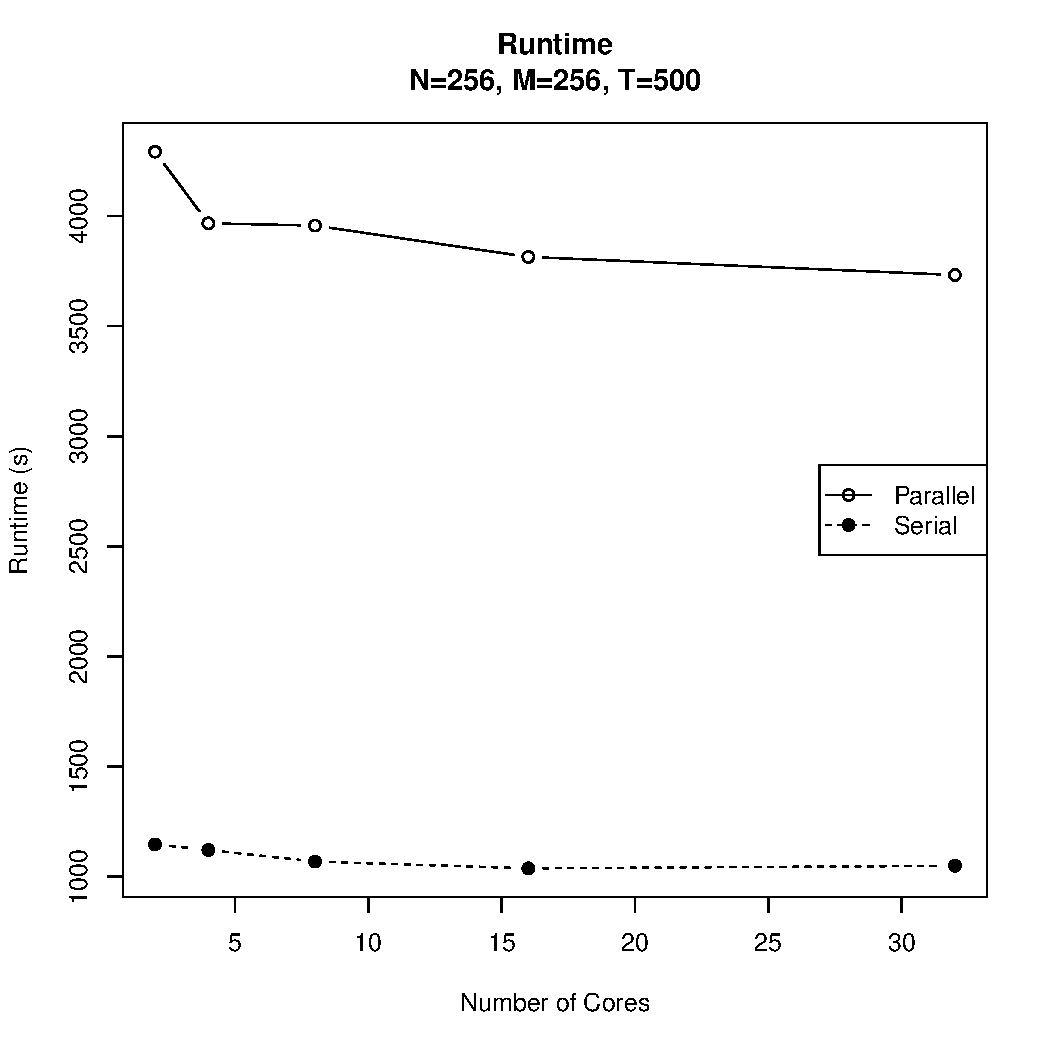
\includegraphics[width=0.6\textwidth]{../figure/runtime-N_256-T_500.pdf}
    \caption{Runtime as a function of number of cores used.}
    \label{fig:runtime-256-500}
\end{figure*}

Figures for other testing conditions are shown in the appendix, in
Figures~\ref{fig:runtime1}--\ref{fig:runtime4}. In general, runtime for the
serial code remains constant, and runtime for the parallel code decreases with
more processors. In many cases, runtime increases when going from 2 to 4
cores---this may represent increased communication cost between more processors.
Noise in our plots may be caused by changes in processing load on the Odyssey
server.

We examined how our implementation scales as we increase the
problem size, especially $N$. A log-log plot of running time vs. $N$ is shown in
Figure~\ref{fig:scaling-16-200}. Judging by the slopes on the graph, our
GraphLab code scales better than the serial code for smaller $N$, but unfortunately not for other values of $N$. 

\begin{figure*}[htb]
    \centering
    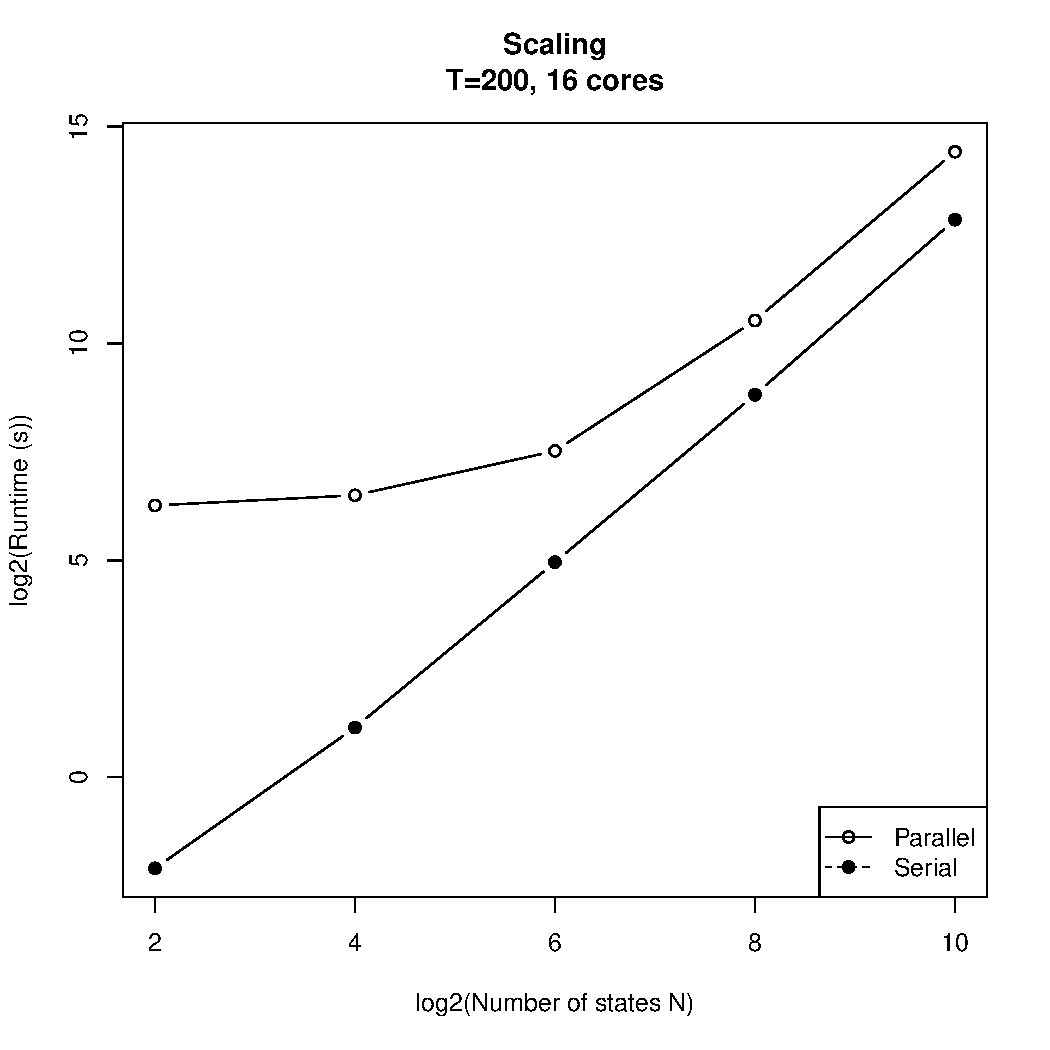
\includegraphics[width=0.6\textwidth]{../figure/scaling-cores_16-T_200.pdf}
    \caption{Log-Log plot of runtime as a function of number of states $N$.}
    \label{fig:scaling-16-200}
\end{figure*}

Additional figures for other testing conditions display similar trends and are
shown in the appendix, Figures~\ref{fig:scaling1}--\ref{fig:scaling4}. 


\section{Conclusion}

Our implementation is awesome


\bibliographystyle{unsrt}
\bibliography{references}

\end{multicols*}

\clearpage
\appendix

\section{Appendix of Figures}

This section includes all of our figures for both runtime and scaling, for all
of the parameters tested. Figures~\ref{fig:runtime1}--\ref{fig:runtime4} show
parallel and serial runtime as a function of the number of cores used, while
Figures~\ref{fig:scaling1}--\ref{fig:scaling4} show log-log plots of runtime as
a function of $N$, the number of hidden states in our HMM. 

\begin{figure}[htb]
    \centering
    $\begin{array}{cc}
    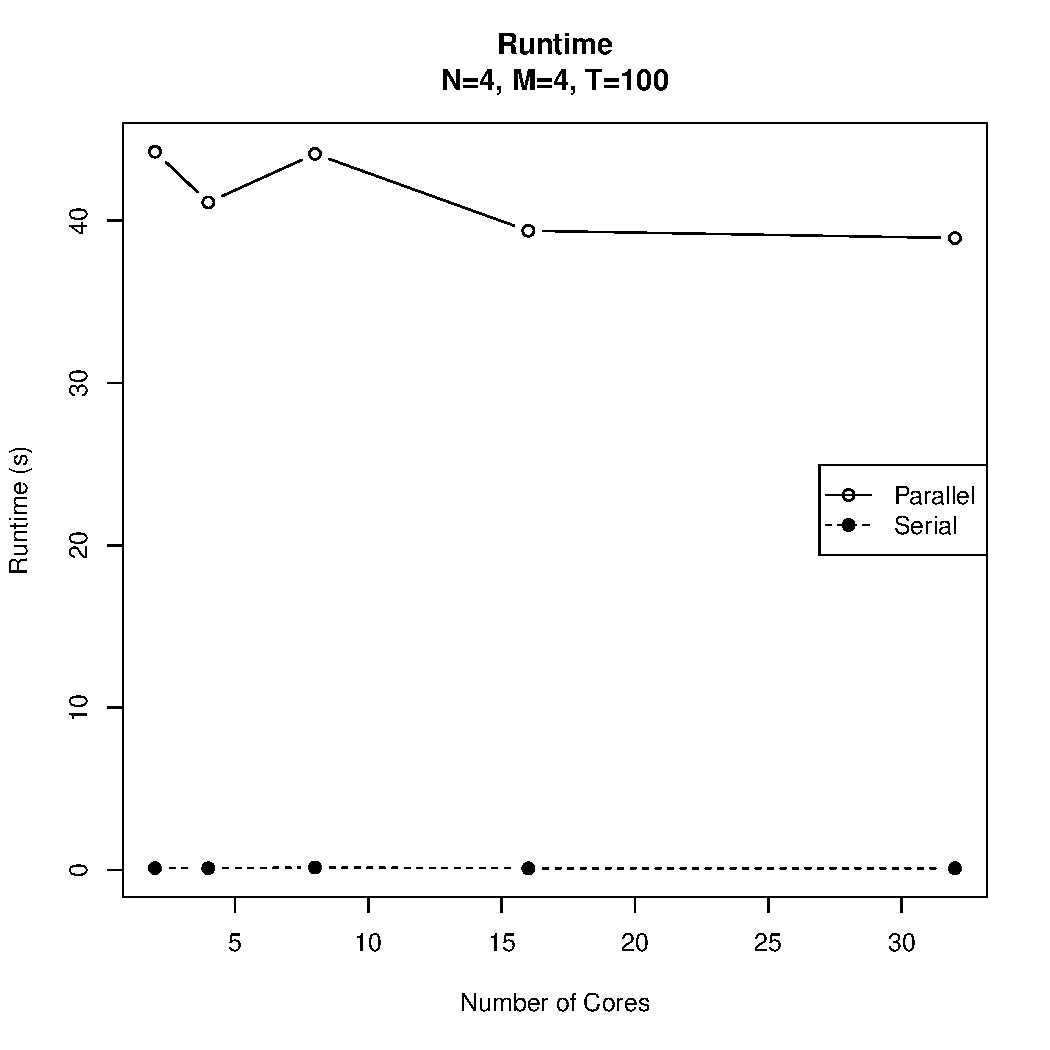
\includegraphics[width=3in]{../figure/runtime-N_4-T_100.pdf} & 
    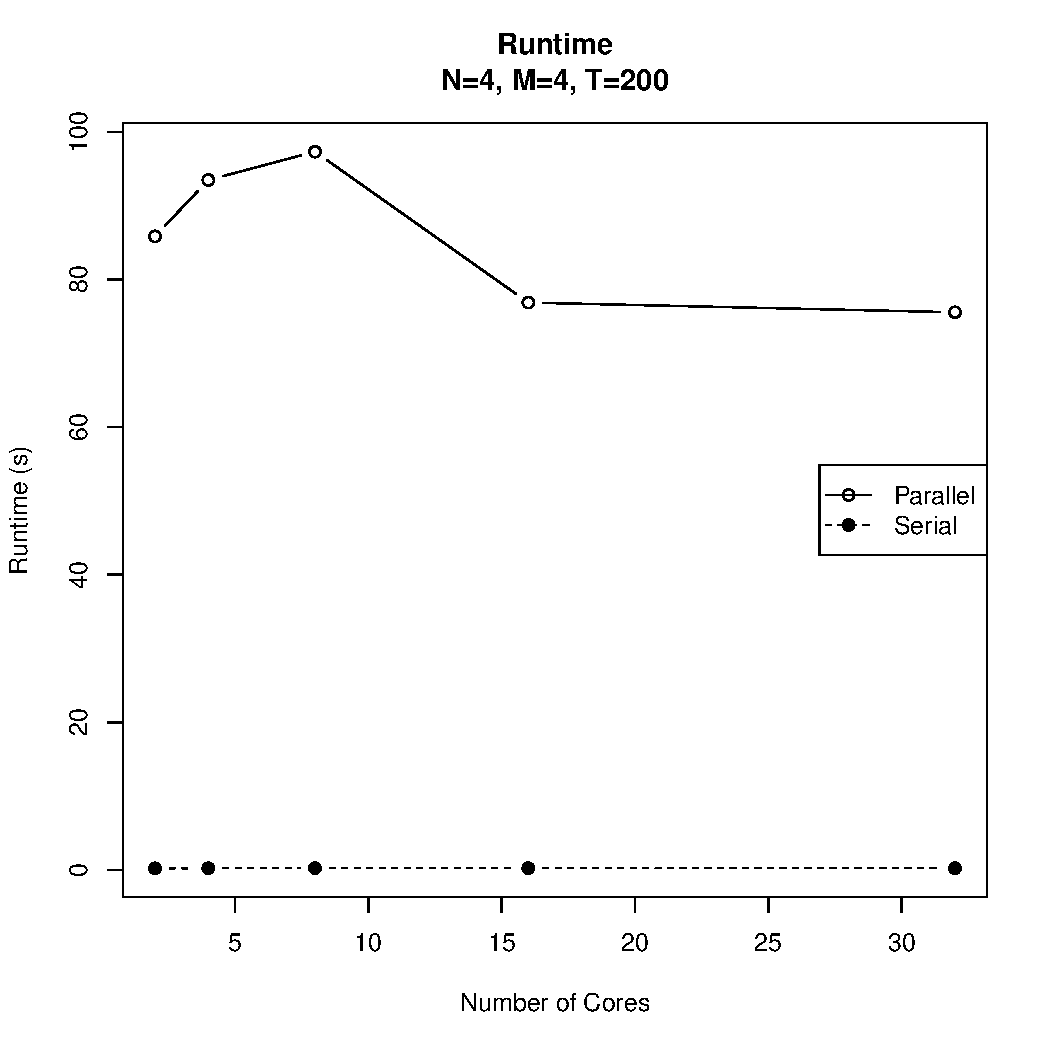
\includegraphics[width=3in]{../figure/runtime-N_4-T_200.pdf} \\
    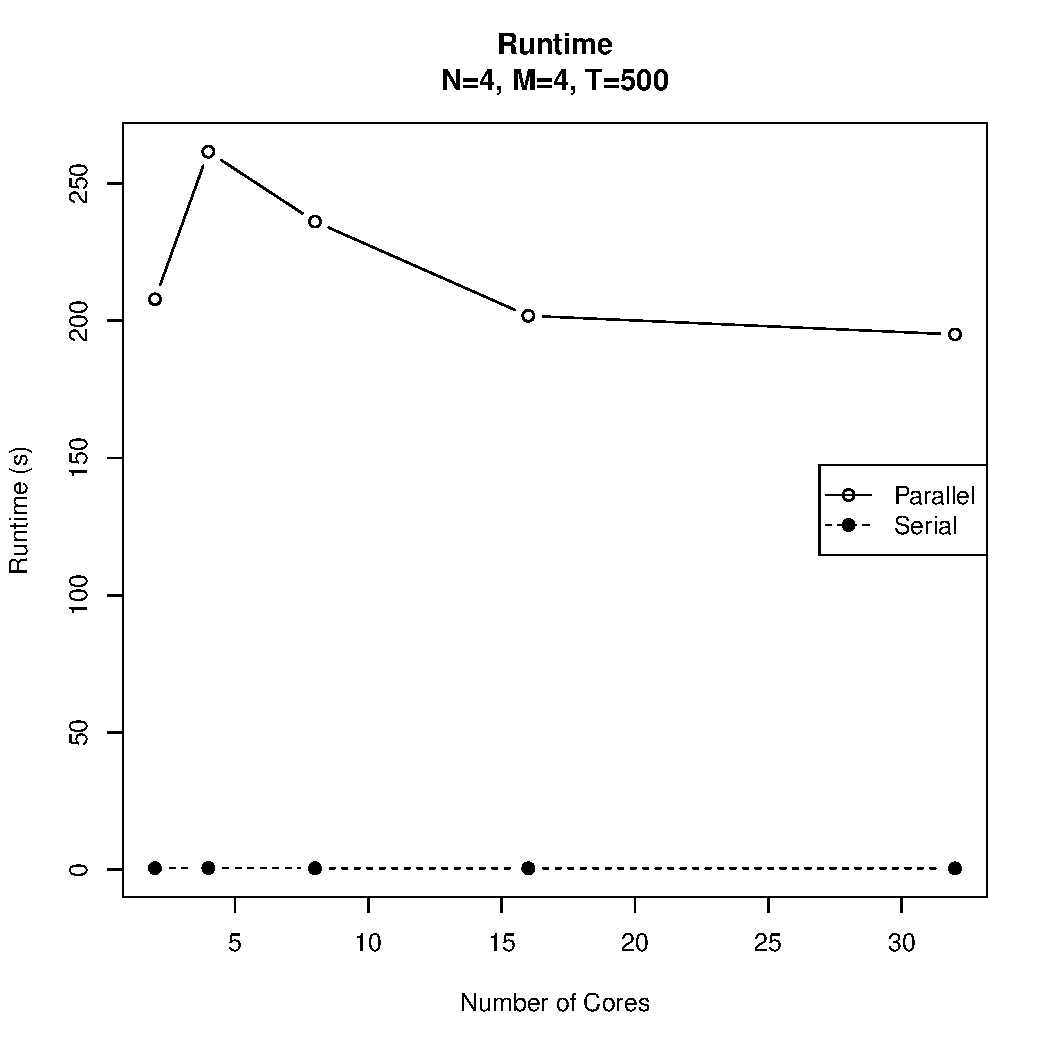
\includegraphics[width=3in]{../figure/runtime-N_4-T_500.pdf} & 
    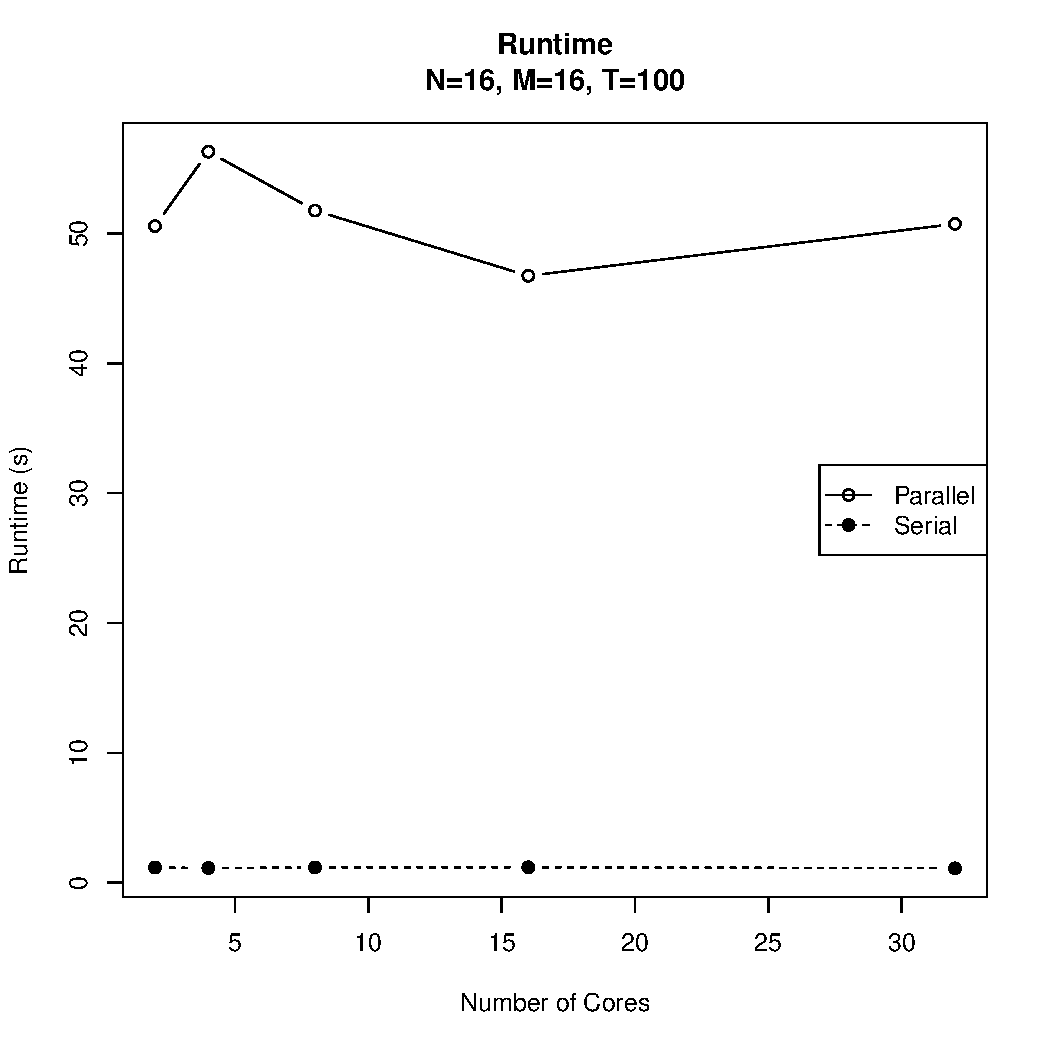
\includegraphics[width=3in]{../figure/runtime-N_16-T_100.pdf} \\
    \end{array}$ 
    \caption{~}
    \label{fig:runtime1}
\end{figure}

\begin{figure}[htb]
    \centering
    $\begin{array}{cc}
    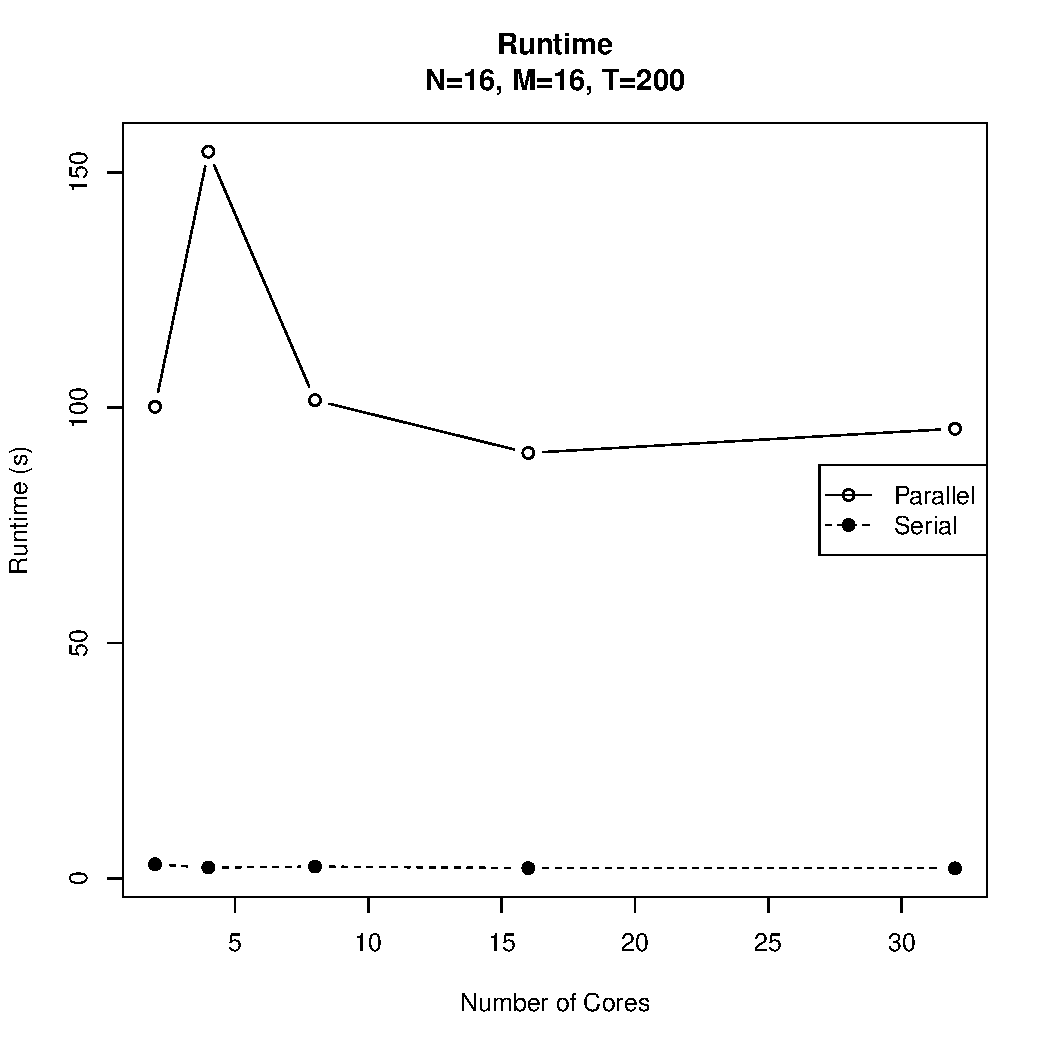
\includegraphics[width=3in]{../figure/runtime-N_16-T_200.pdf} & 
    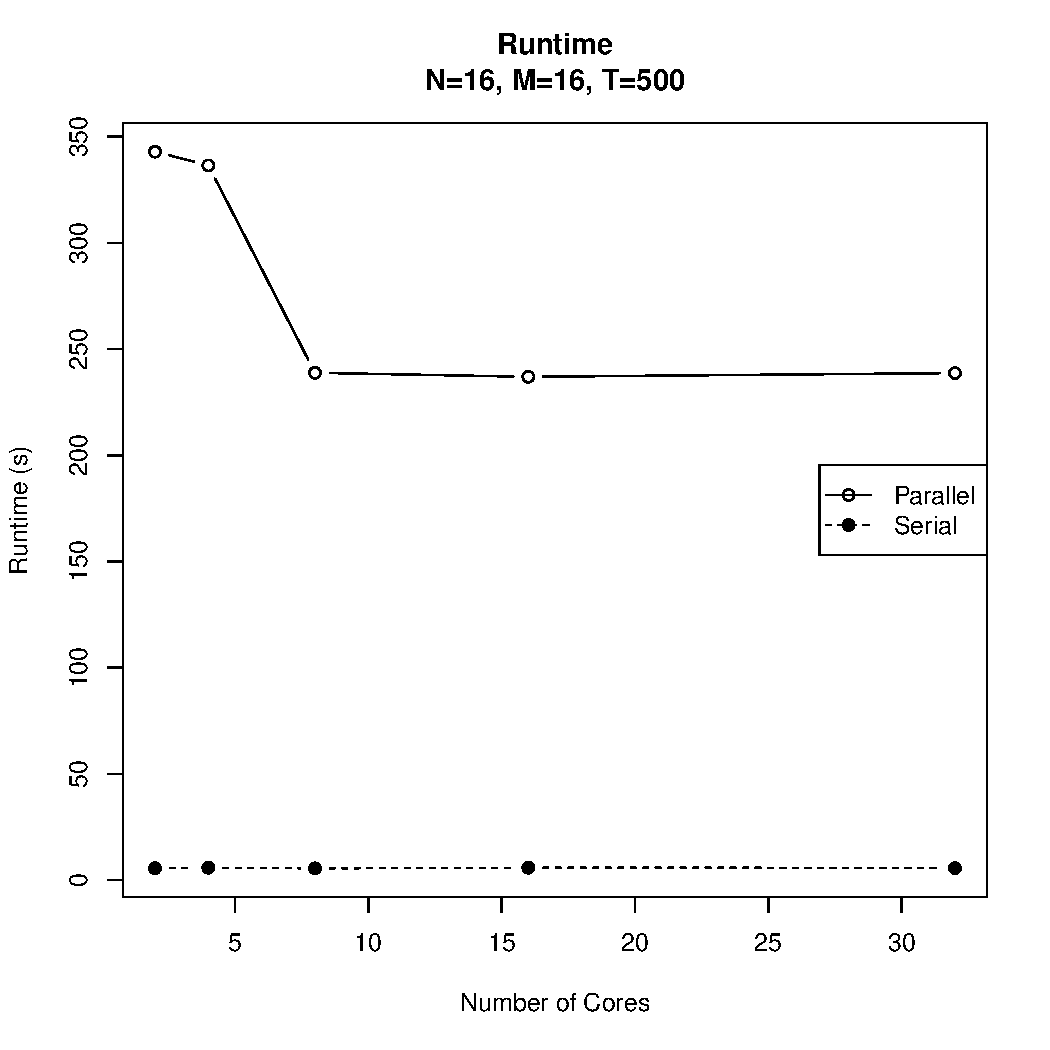
\includegraphics[width=3in]{../figure/runtime-N_16-T_500.pdf} \\
    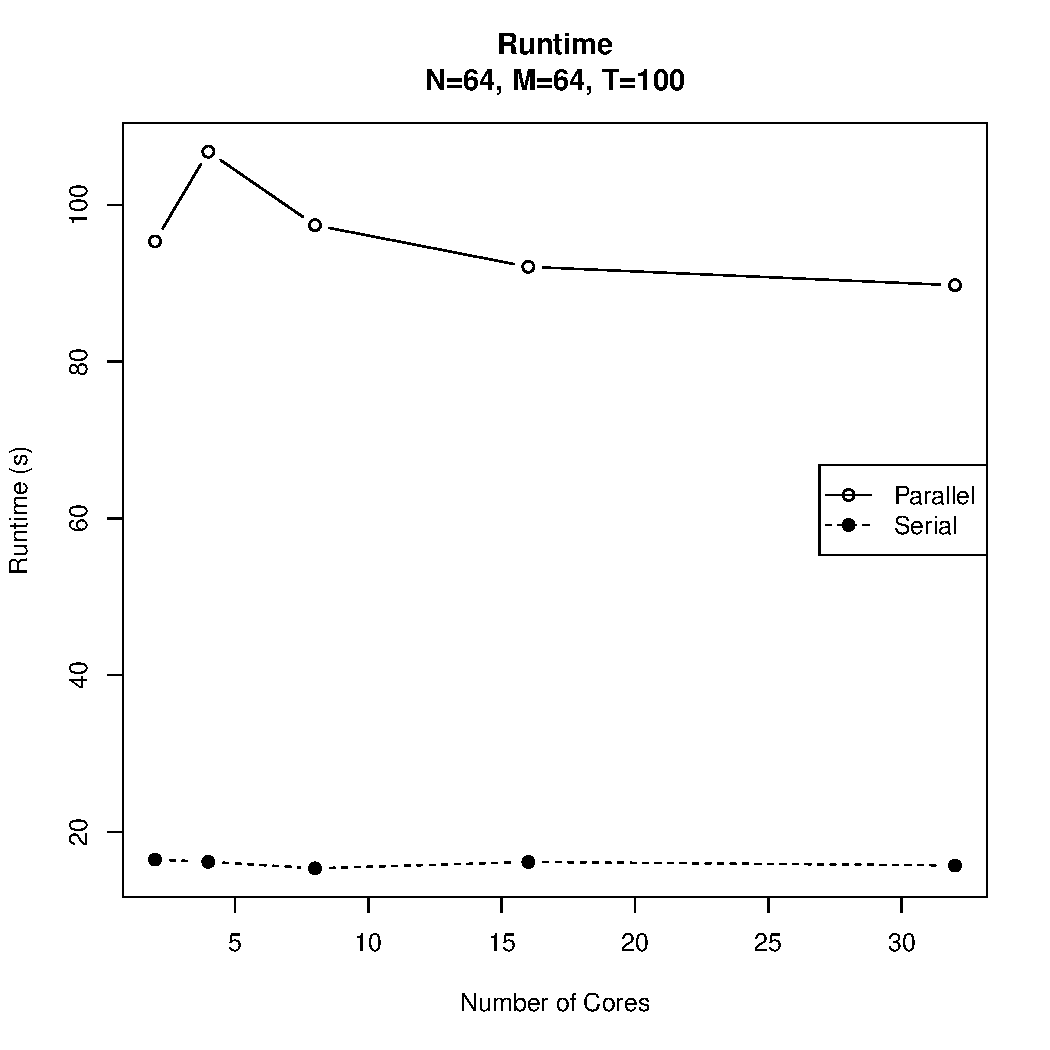
\includegraphics[width=3in]{../figure/runtime-N_64-T_100.pdf} & 
    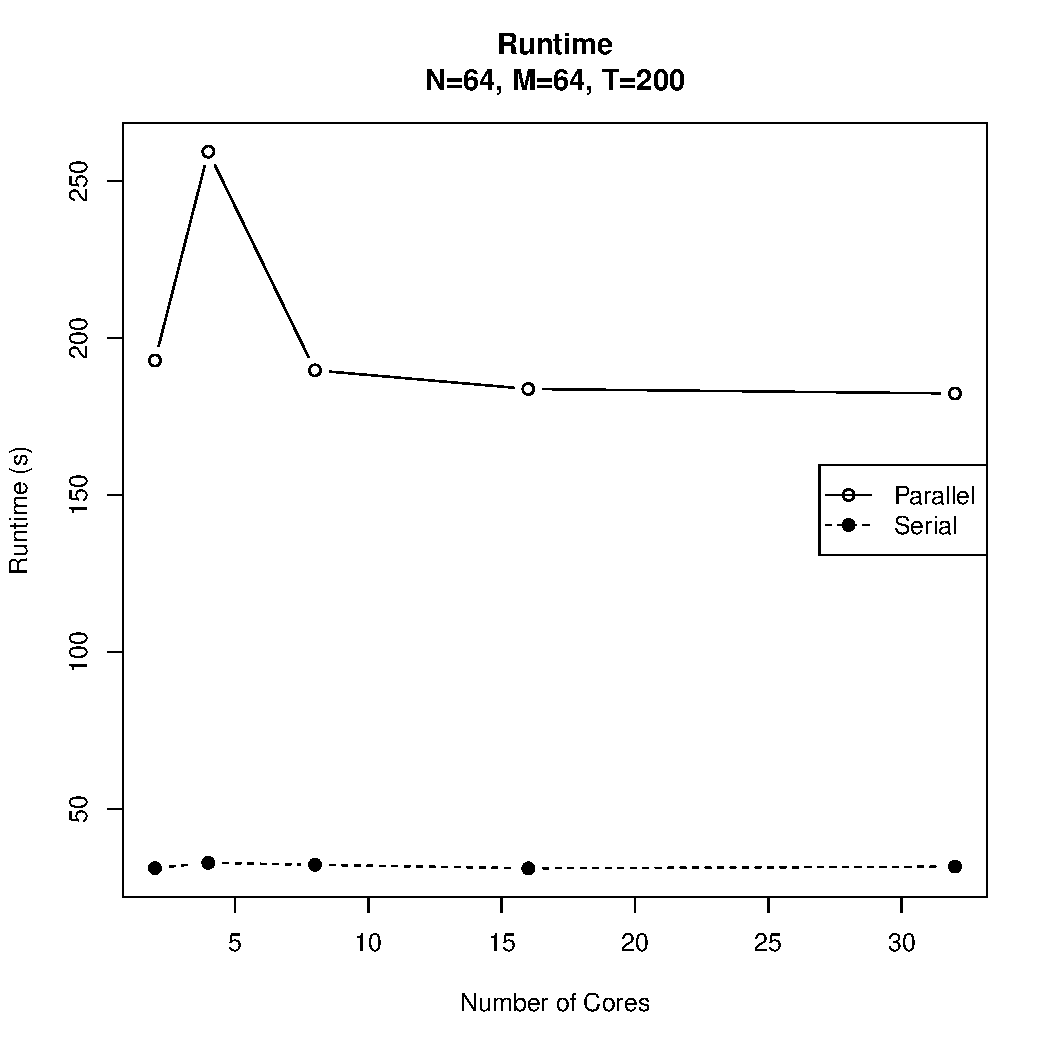
\includegraphics[width=3in]{../figure/runtime-N_64-T_200.pdf} \\
    \end{array}$ 
    \caption{~}
    \label{fig:runtime2}
\end{figure}

\begin{figure}[htb]
    \centering
    $\begin{array}{cc}
    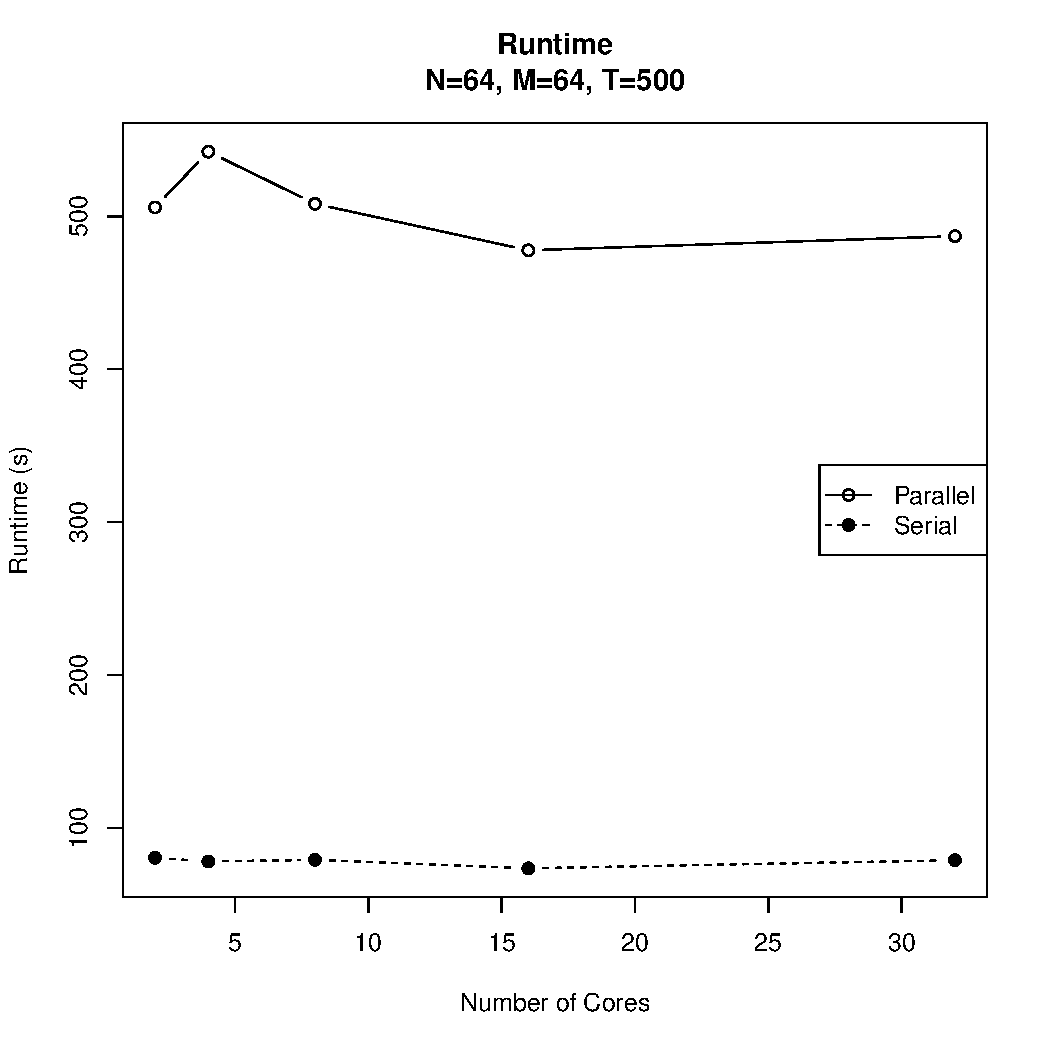
\includegraphics[width=3in]{../figure/runtime-N_64-T_500.pdf} & 
    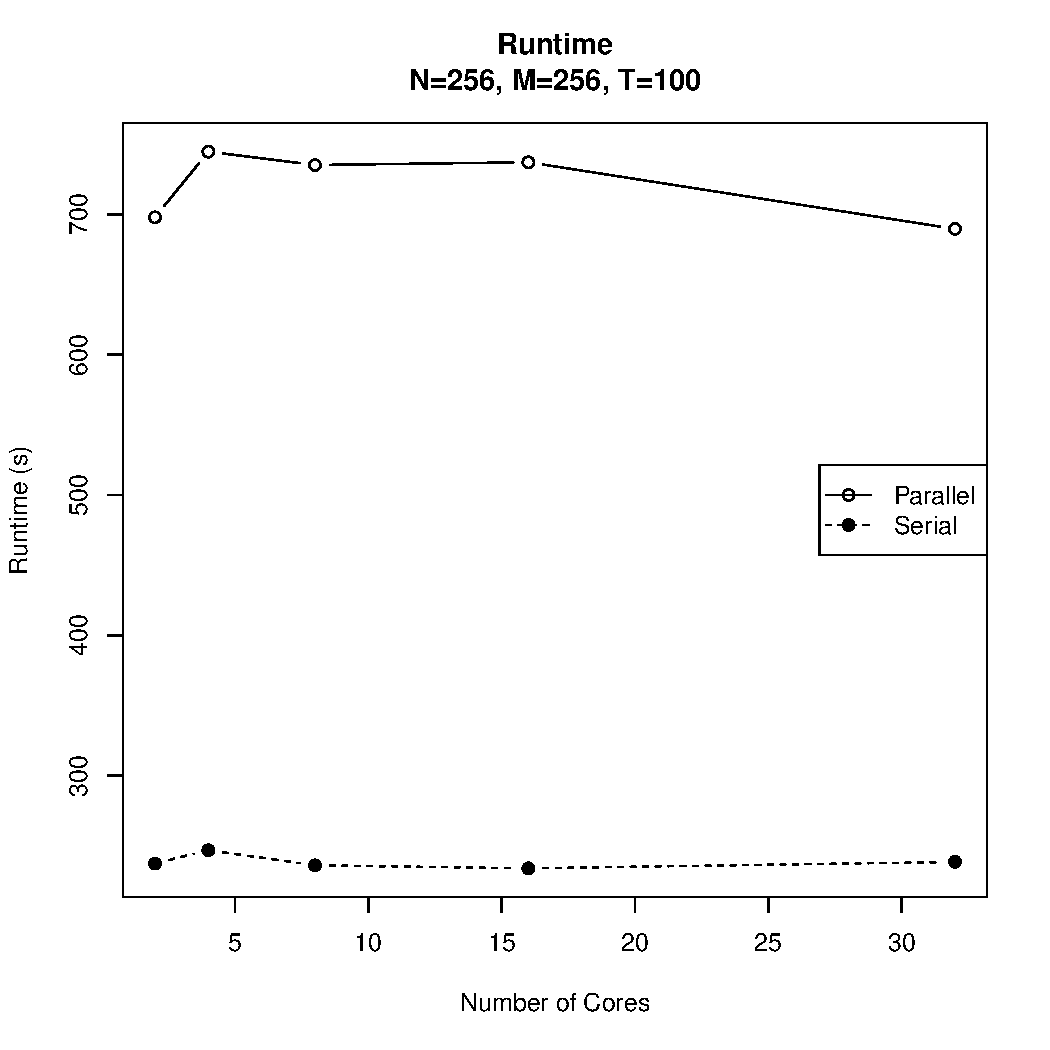
\includegraphics[width=3in]{../figure/runtime-N_256-T_100.pdf} \\
    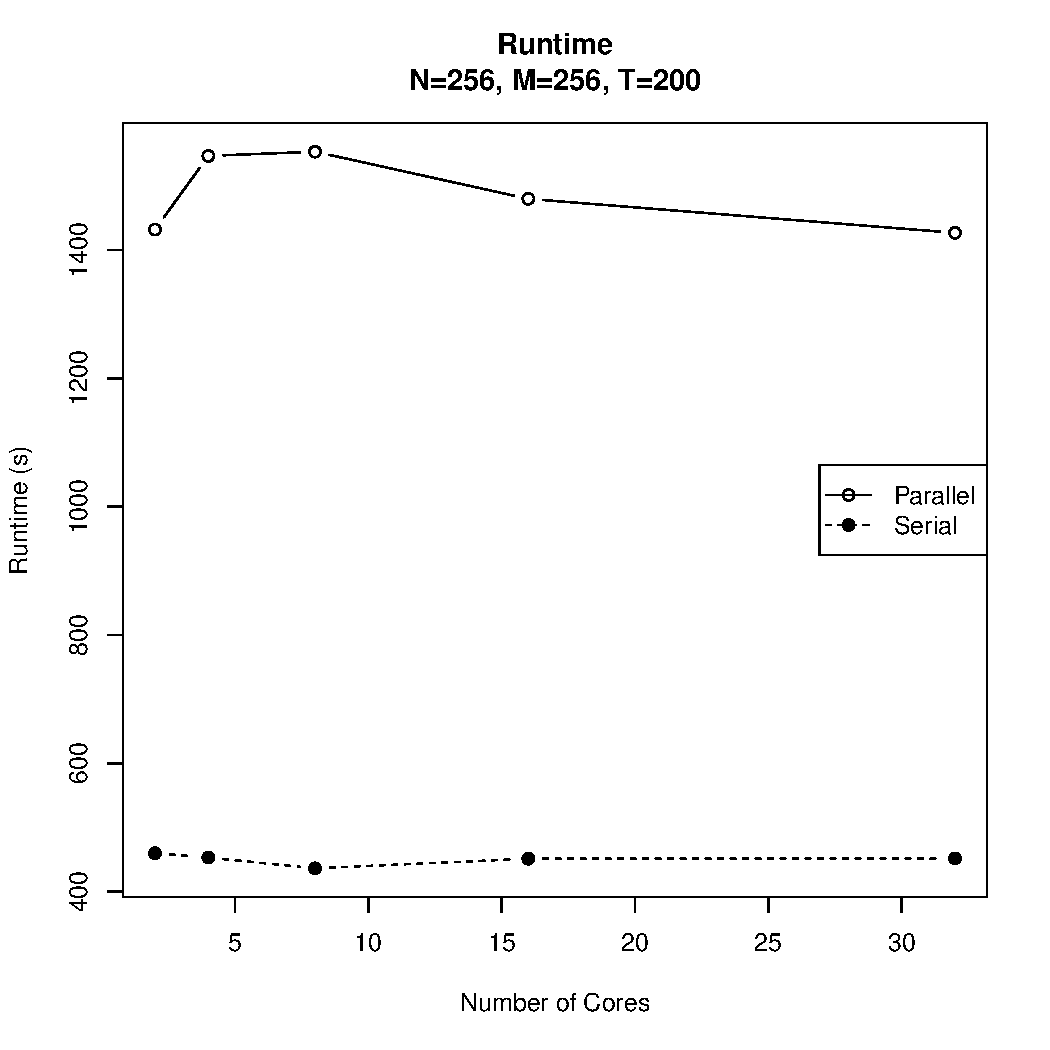
\includegraphics[width=3in]{../figure/runtime-N_256-T_200.pdf} & 
    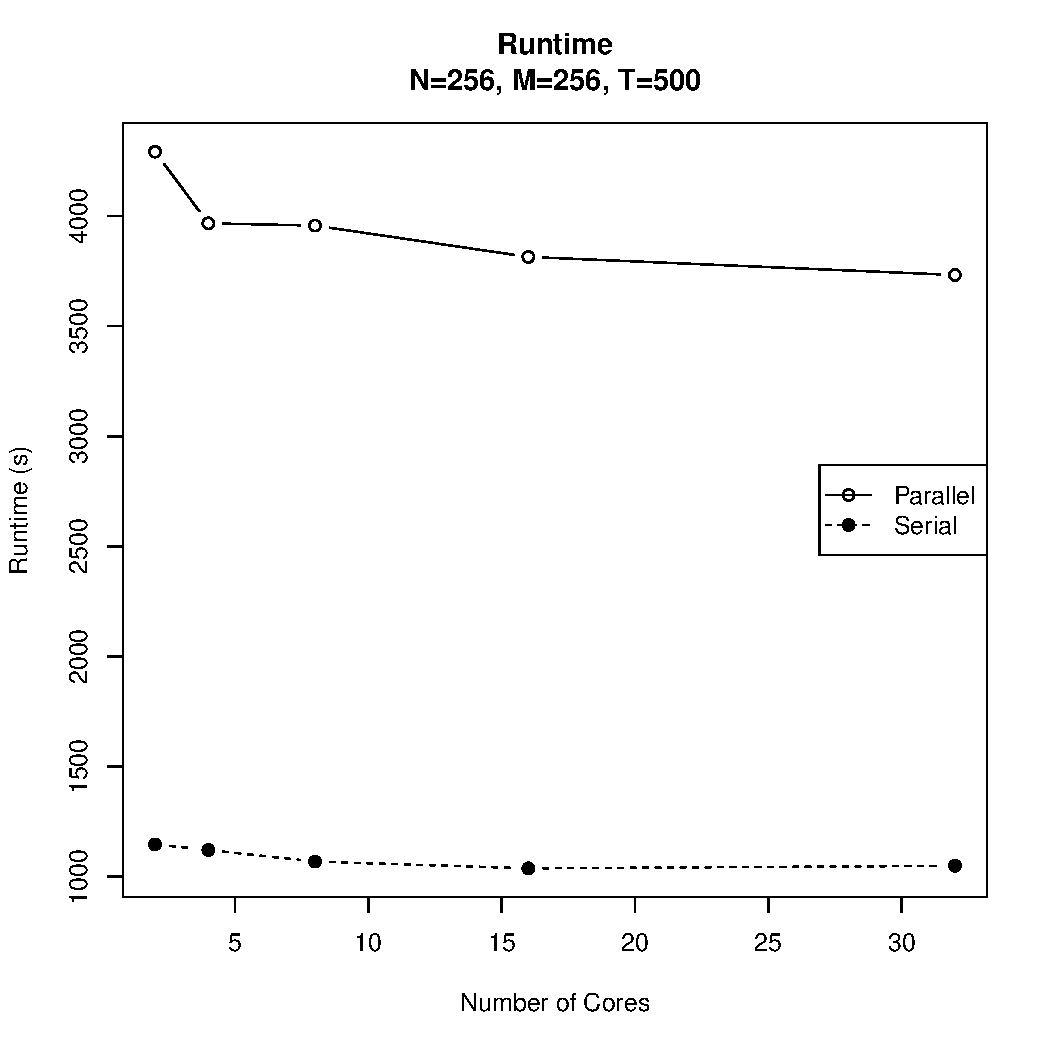
\includegraphics[width=3in]{../figure/runtime-N_256-T_500.pdf} \\
    \end{array}$ 
    \caption{~}
    \label{fig:runtime3}
\end{figure}

\begin{figure}[htb]
    \centering
    $\begin{array}{cc}
    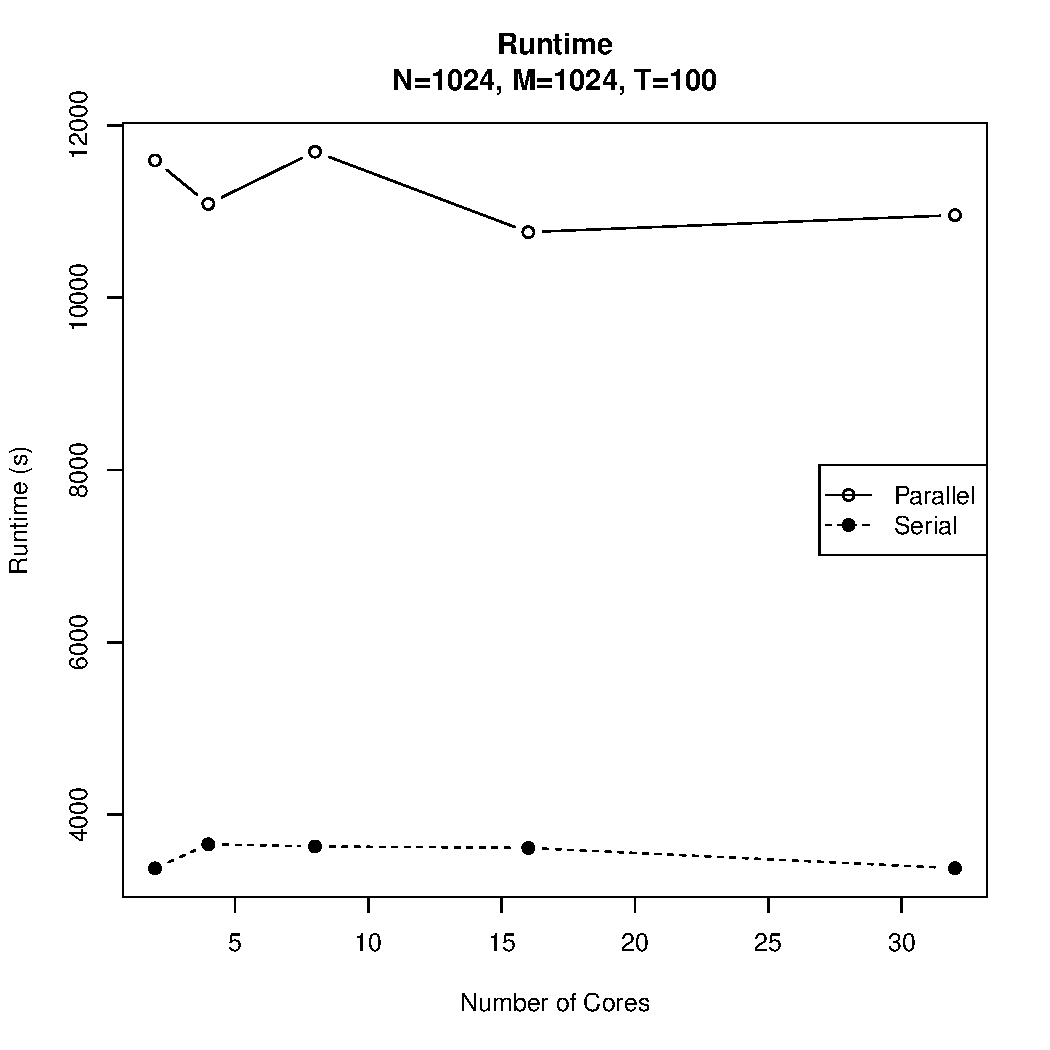
\includegraphics[width=3in]{../figure/runtime-N_1024-T_100.pdf} & 
    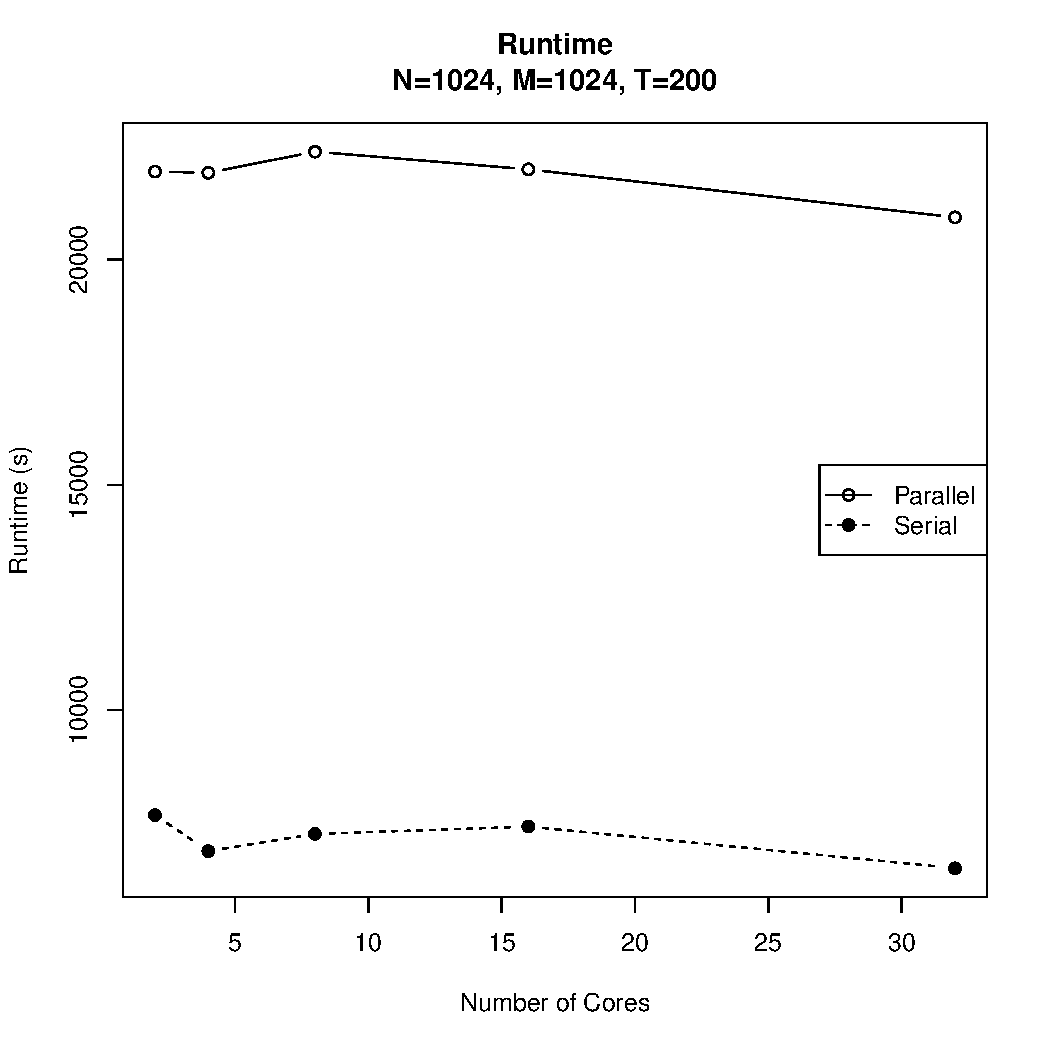
\includegraphics[width=3in]{../figure/runtime-N_1024-T_200.pdf} \\
    \end{array}$ 
    \caption{~}
    \label{fig:runtime4}
\end{figure}

\begin{figure}[htb]
    \centering
    $\begin{array}{cc}
    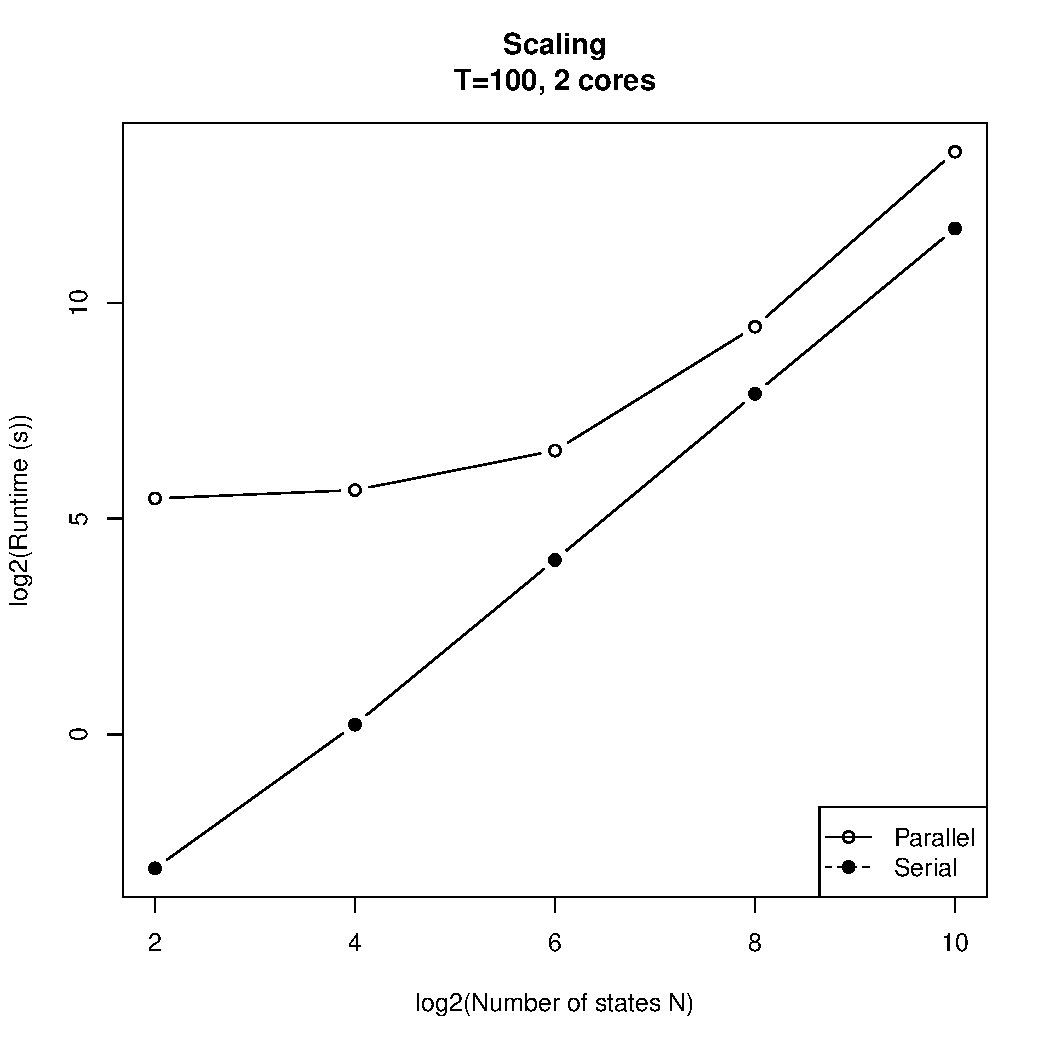
\includegraphics[width=3in]{../figure/scaling-cores_2-T_100.pdf} & 
    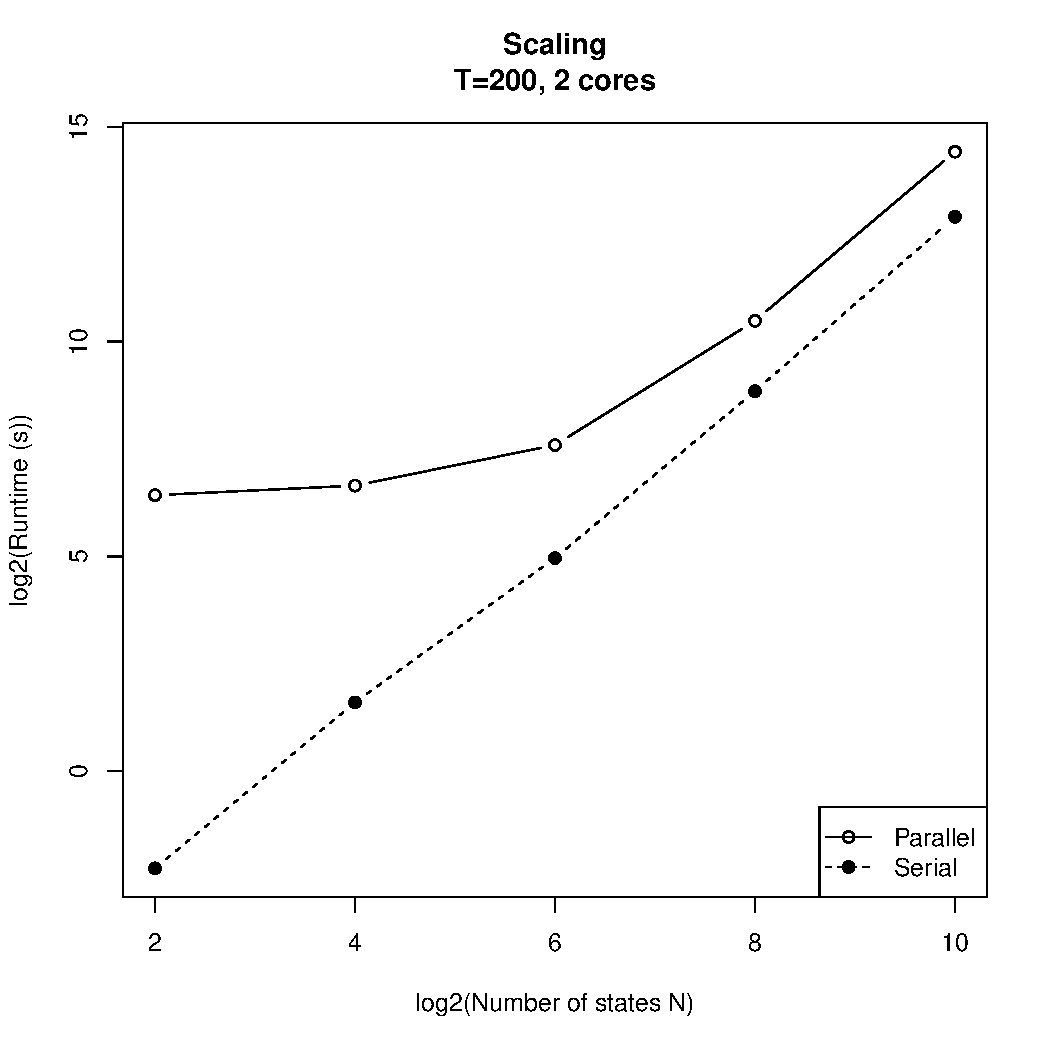
\includegraphics[width=3in]{../figure/scaling-cores_2-T_200.pdf} \\
    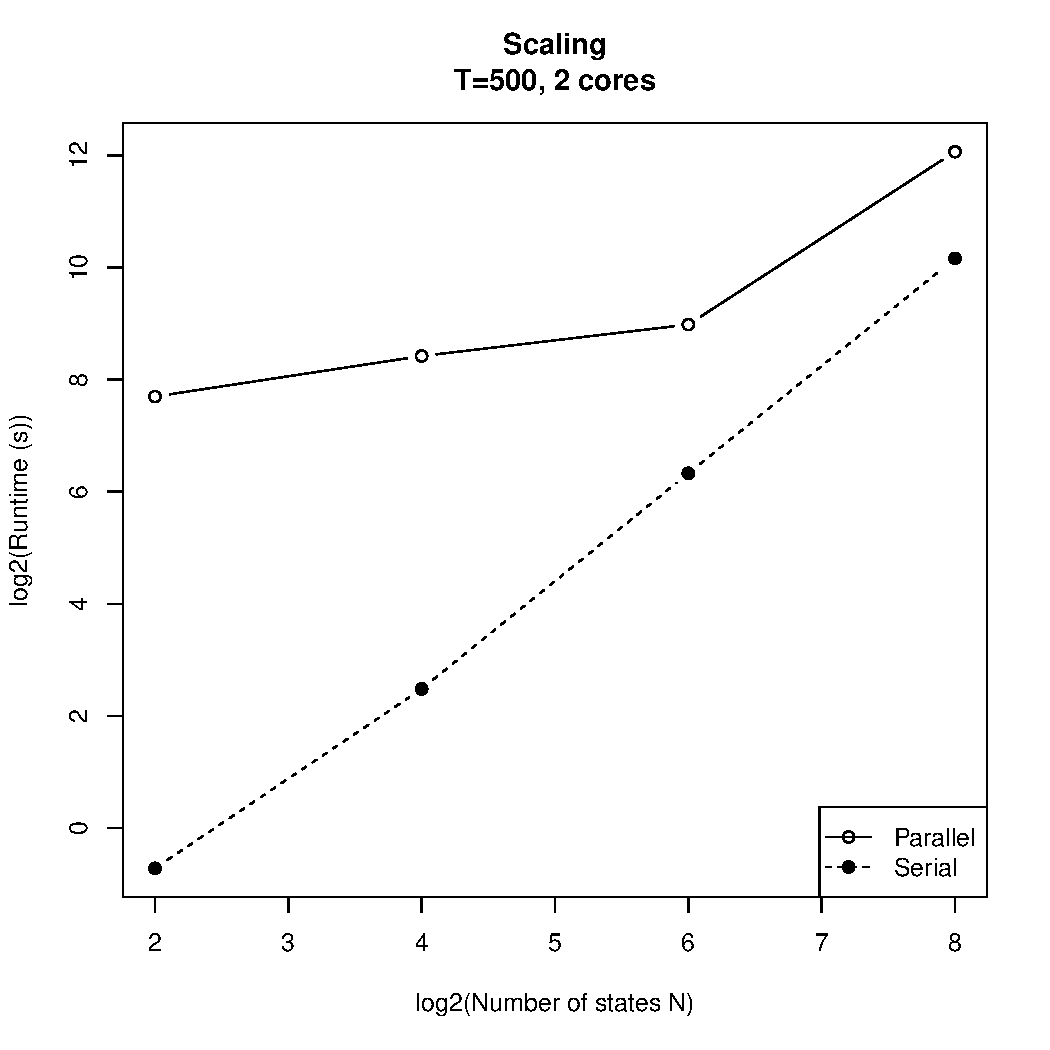
\includegraphics[width=3in]{../figure/scaling-cores_2-T_500.pdf} & 
    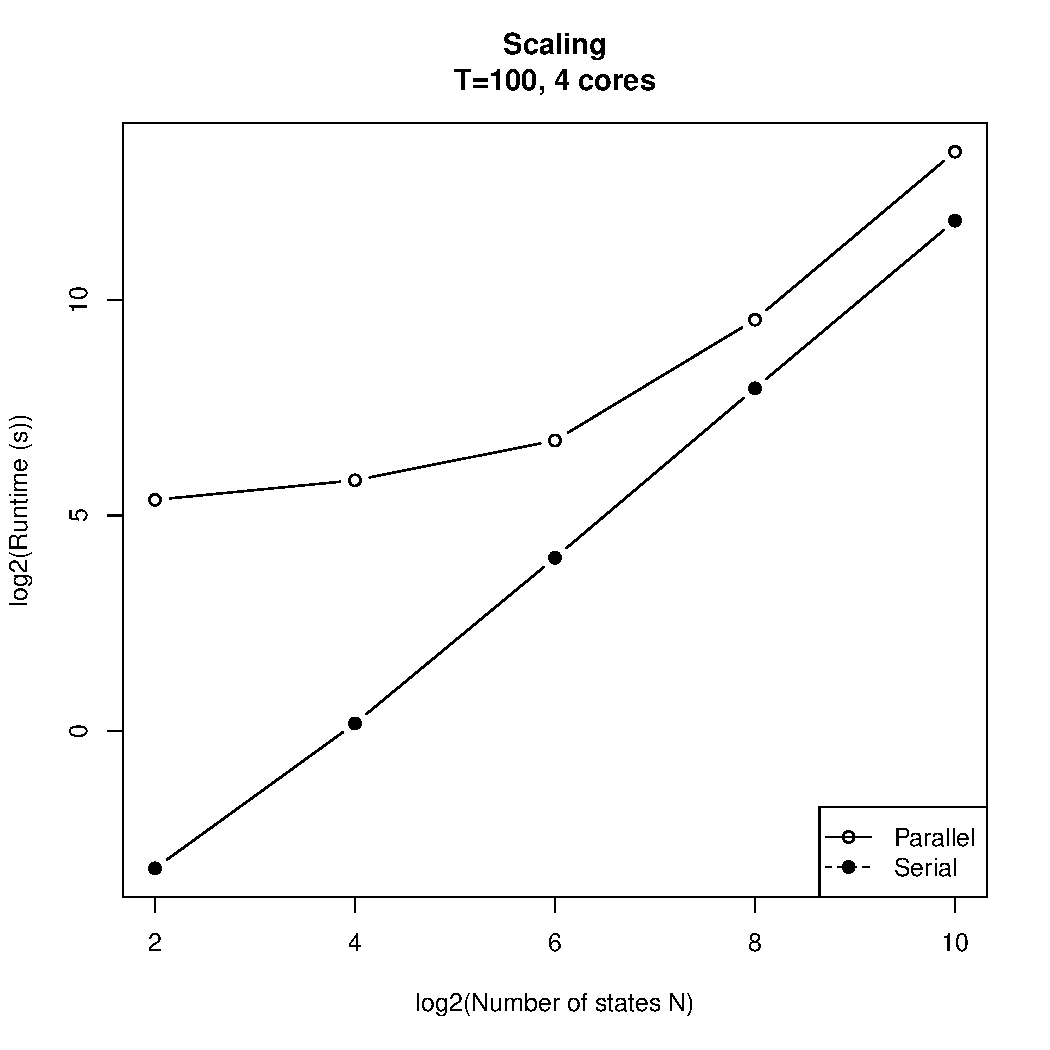
\includegraphics[width=3in]{../figure/scaling-cores_4-T_100.pdf} \\
    \end{array}$ 
    \caption{~}
    \label{fig:scaling1}
\end{figure}

\begin{figure}[htb]
    \centering
    $\begin{array}{cc}
    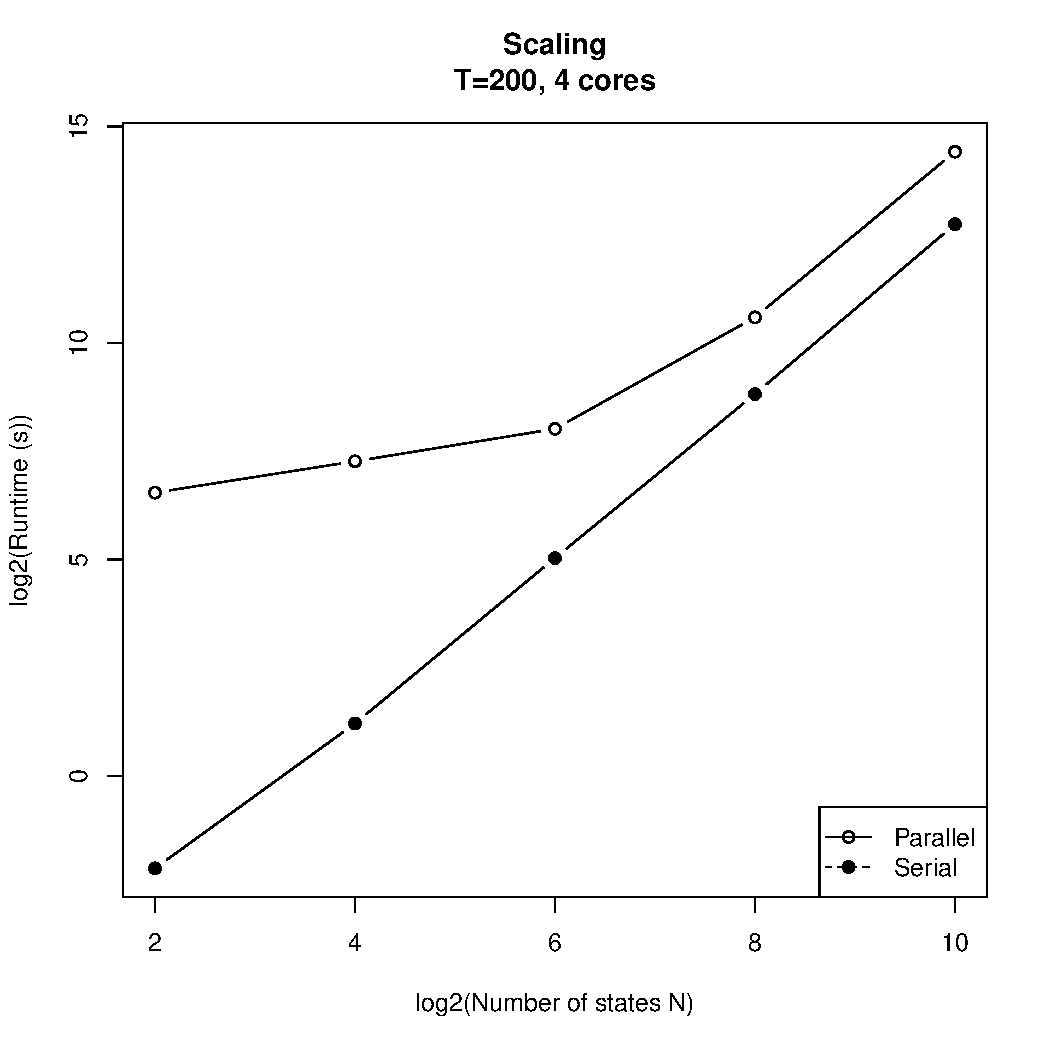
\includegraphics[width=3in]{../figure/scaling-cores_4-T_200.pdf} & 
    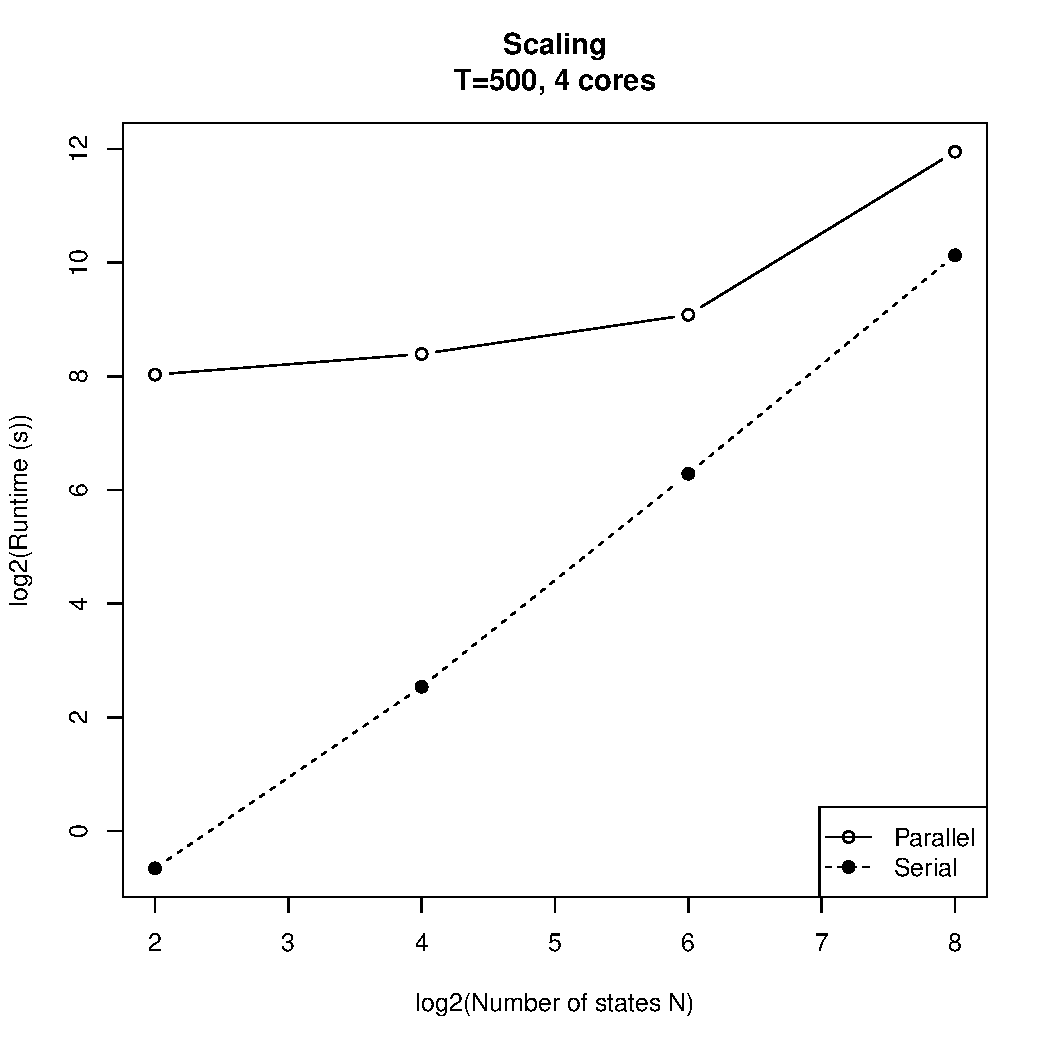
\includegraphics[width=3in]{../figure/scaling-cores_4-T_500.pdf} \\
    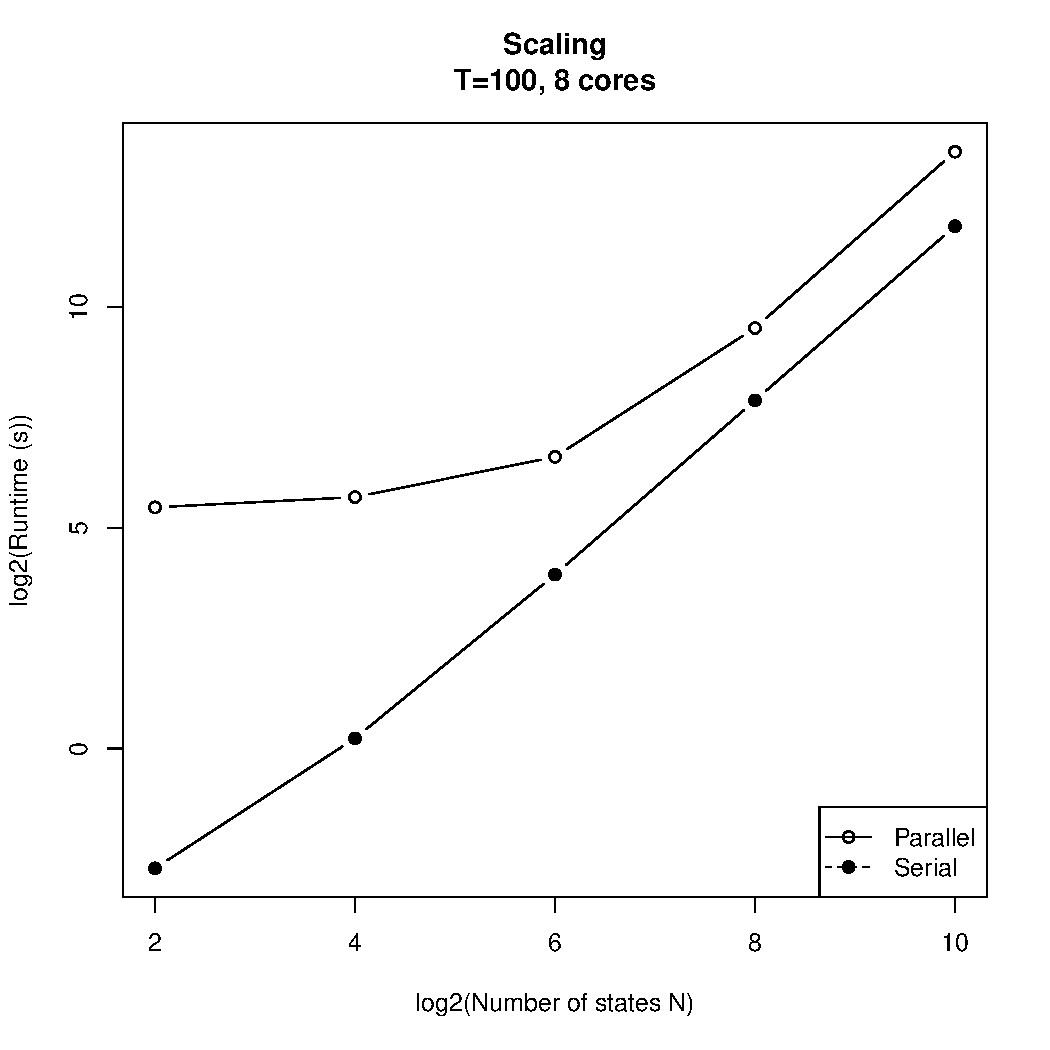
\includegraphics[width=3in]{../figure/scaling-cores_8-T_100.pdf} & 
    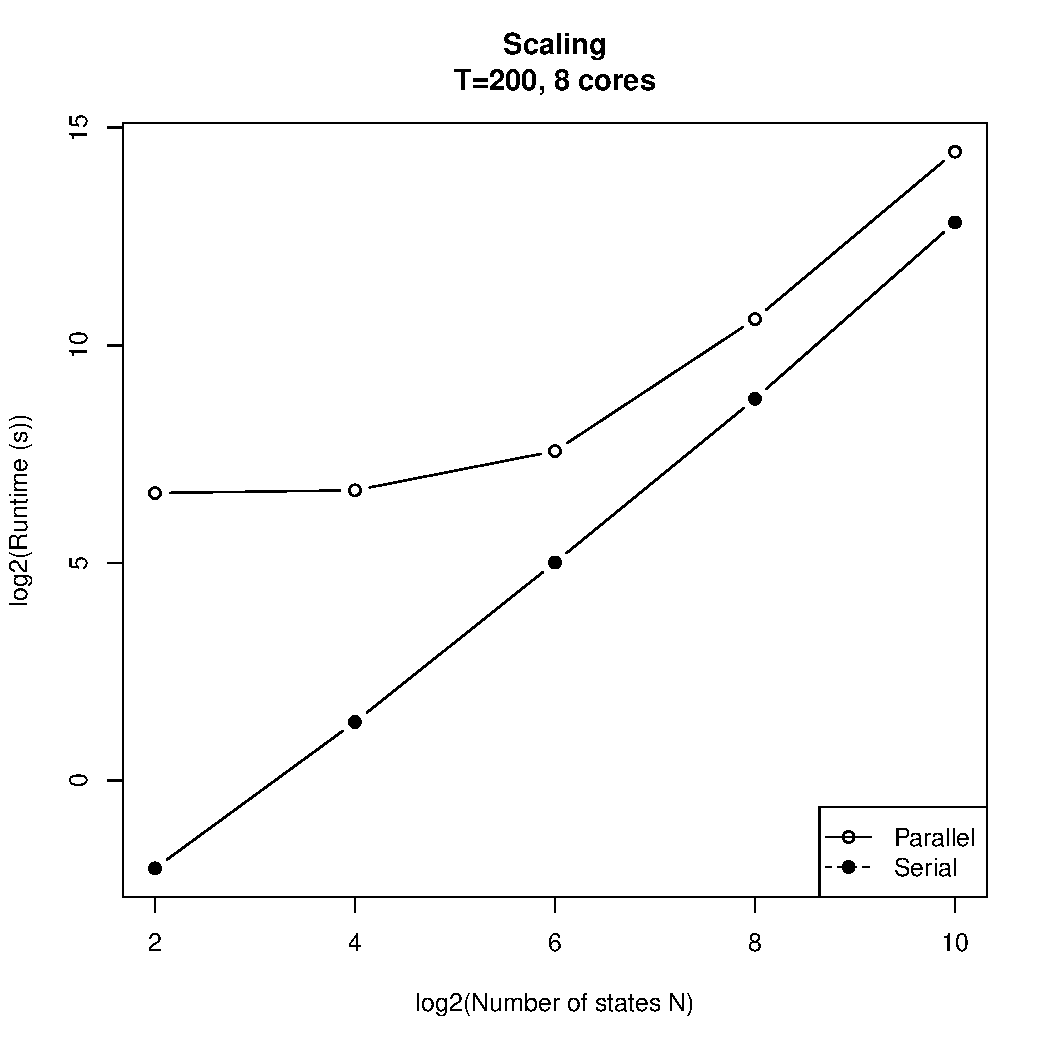
\includegraphics[width=3in]{../figure/scaling-cores_8-T_200.pdf} \\
    \end{array}$ 
    \caption{~}
    \label{fig:scaling2}
\end{figure}

\begin{figure}[htb]
    \centering
    $\begin{array}{cc}
    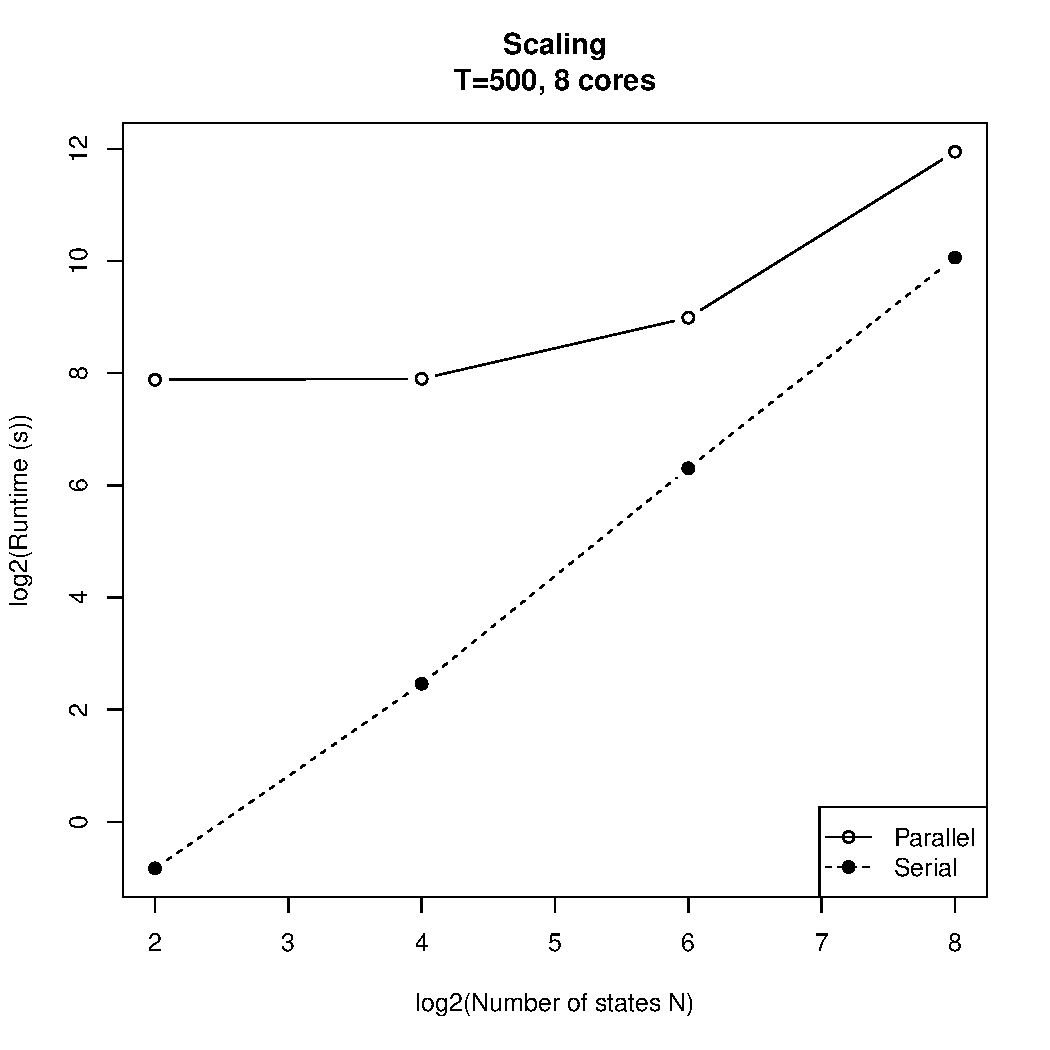
\includegraphics[width=3in]{../figure/scaling-cores_8-T_500.pdf} & 
    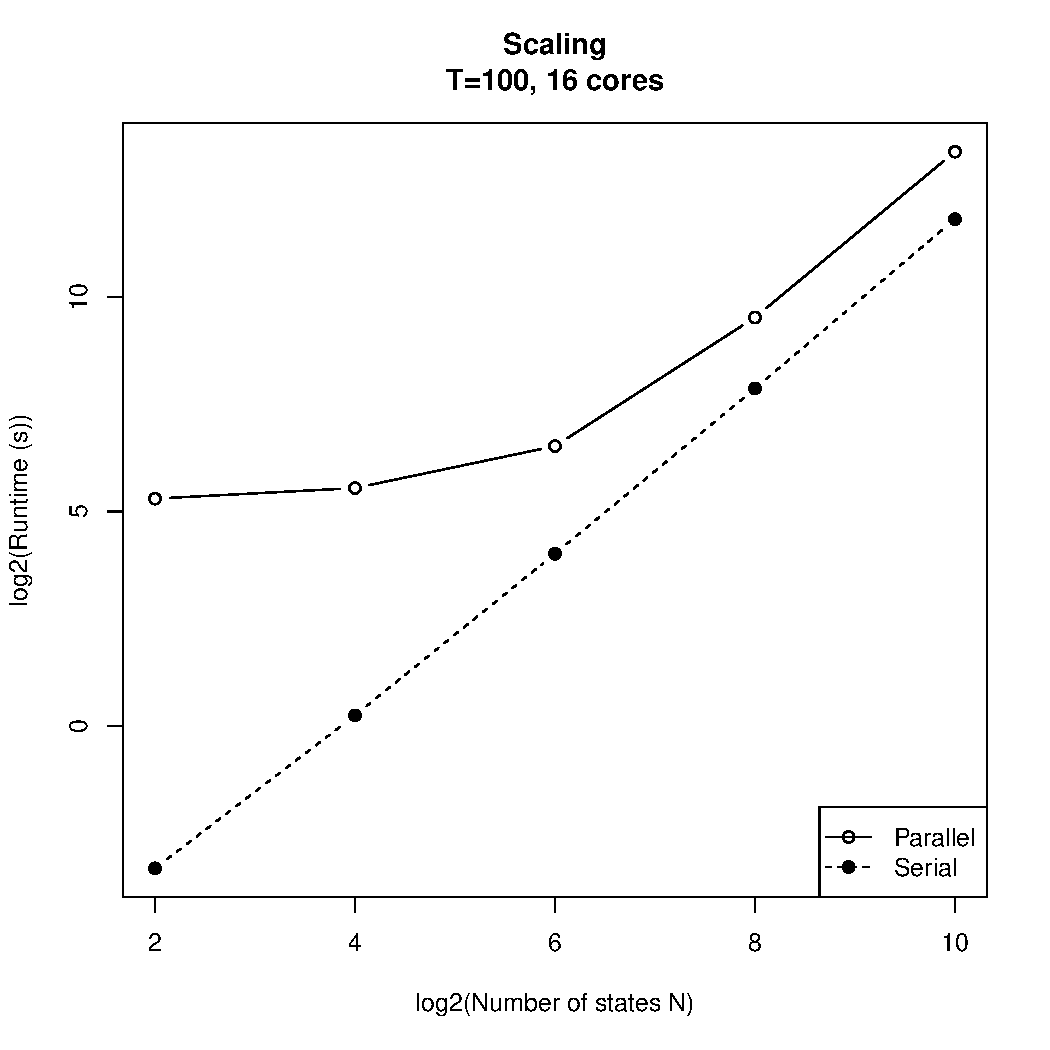
\includegraphics[width=3in]{../figure/scaling-cores_16-T_100.pdf} \\
    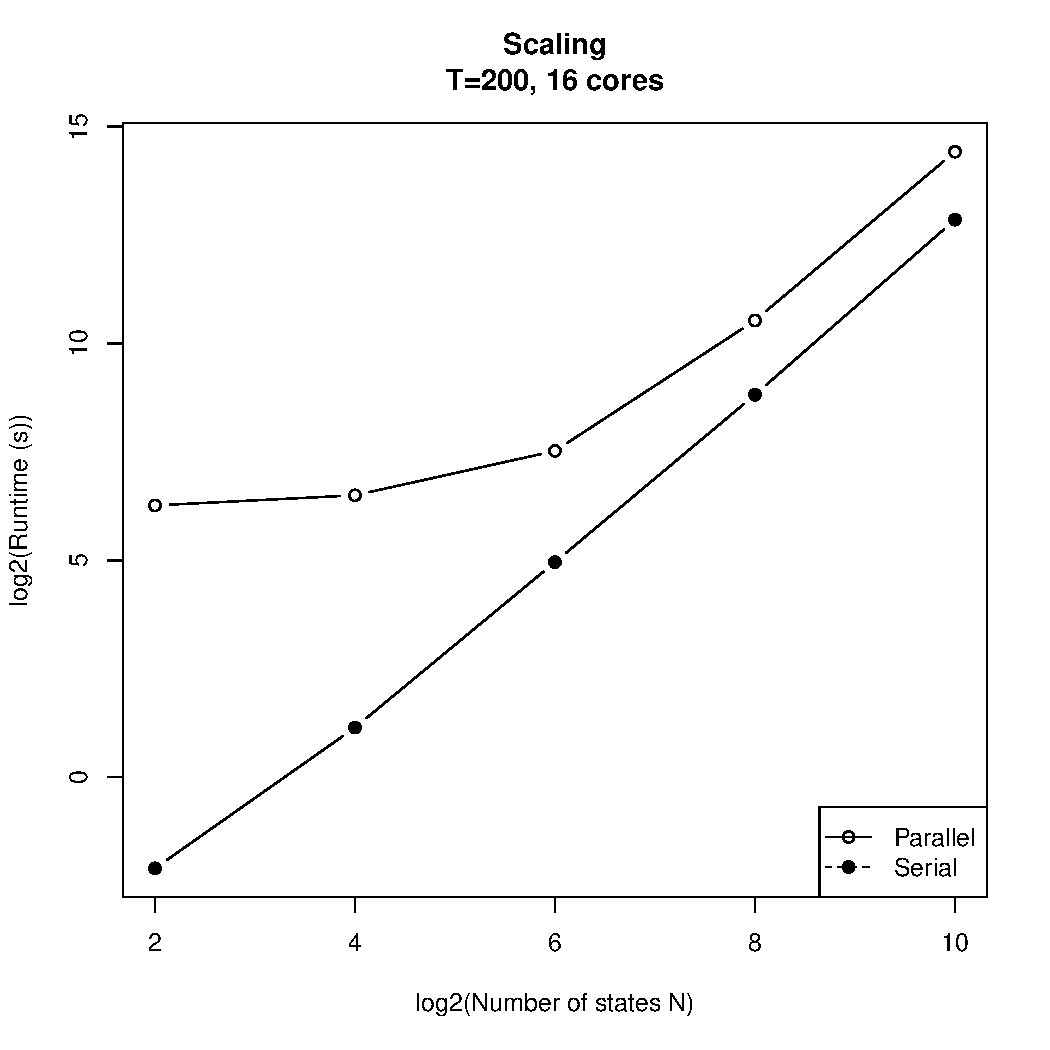
\includegraphics[width=3in]{../figure/scaling-cores_16-T_200.pdf} & 
    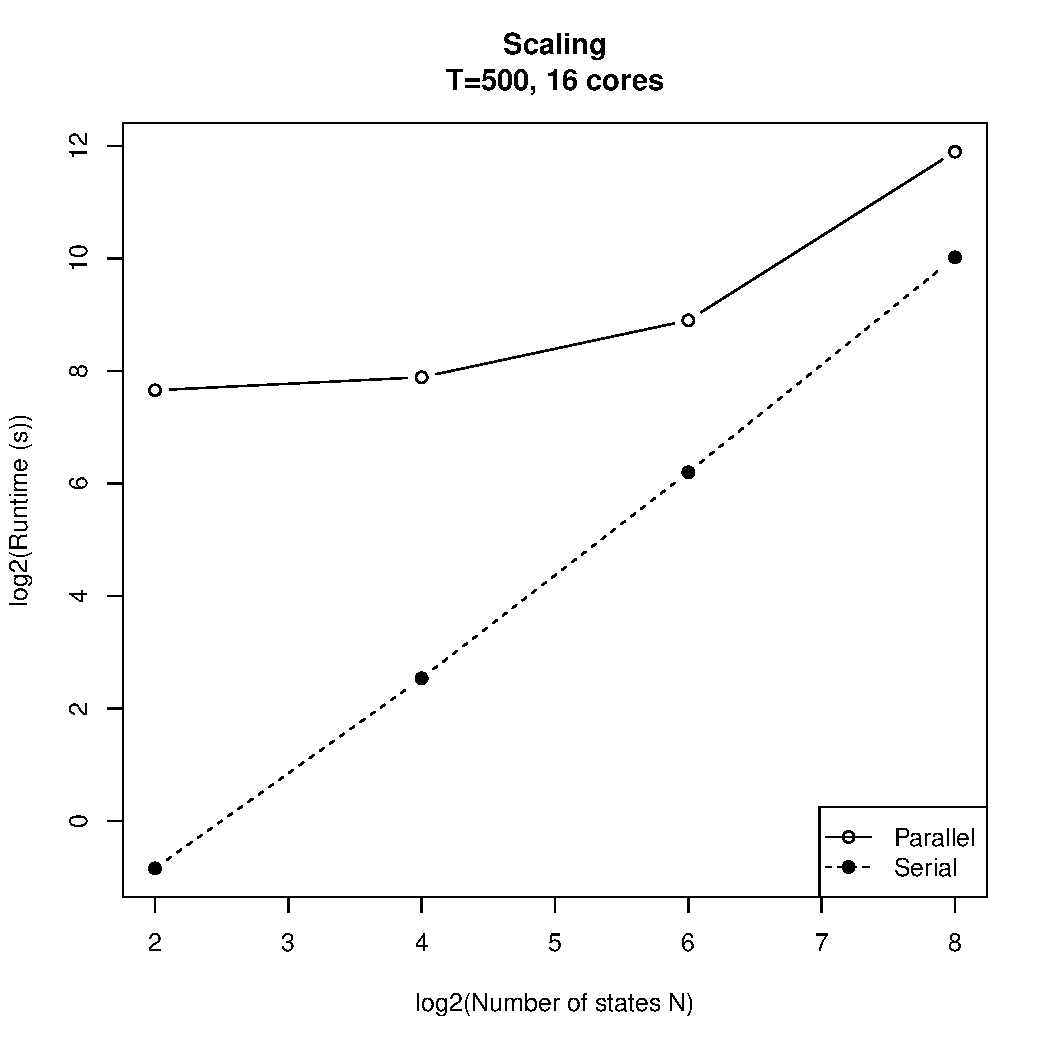
\includegraphics[width=3in]{../figure/scaling-cores_16-T_500.pdf} \\
    \end{array}$ 
    \caption{~}
    \label{fig:scaling3}
\end{figure}

\begin{figure}[htb]
    \centering
    $\begin{array}{cc}
    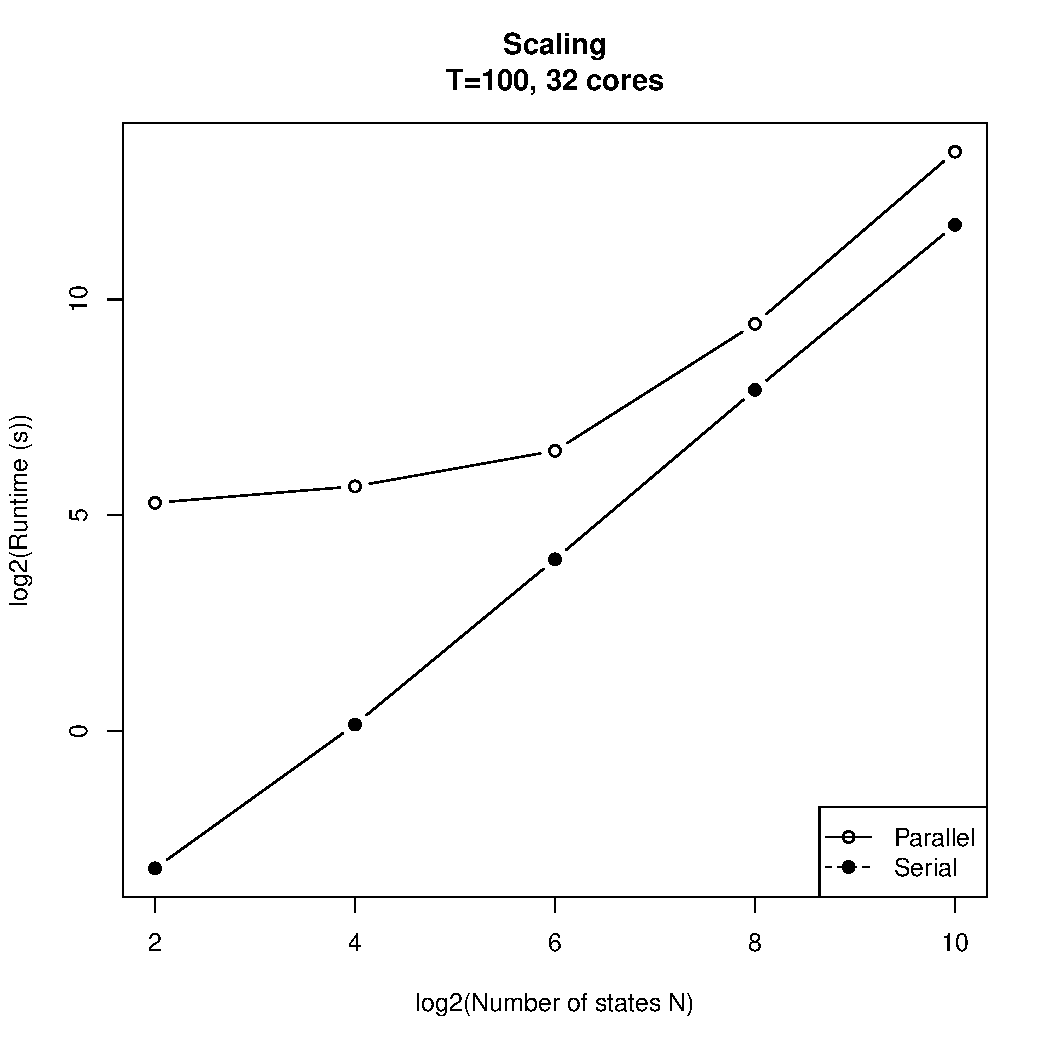
\includegraphics[width=3in]{../figure/scaling-cores_32-T_100.pdf} & 
    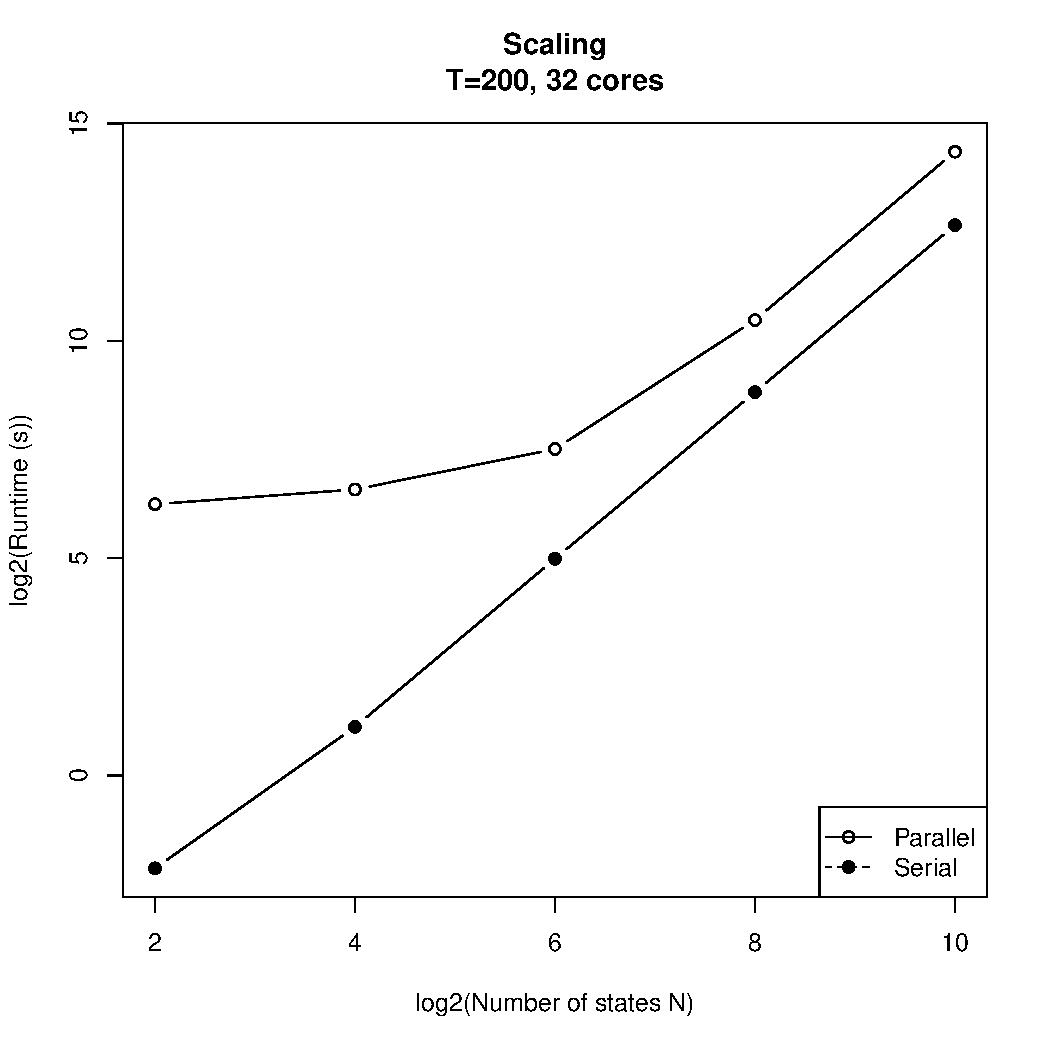
\includegraphics[width=3in]{../figure/scaling-cores_32-T_200.pdf} \\
    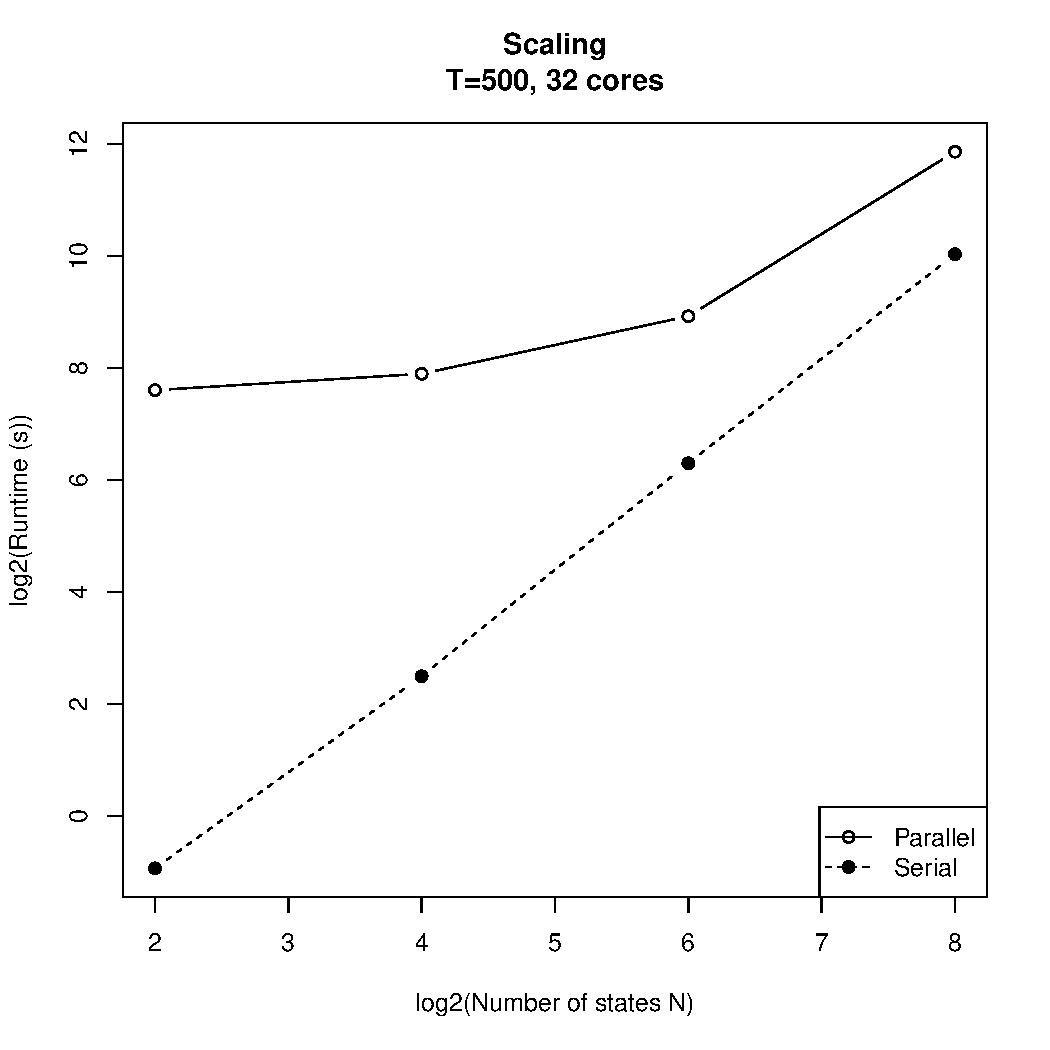
\includegraphics[width=3in]{../figure/scaling-cores_32-T_500.pdf} &
    \end{array}$ 
    \caption{~}
    \label{fig:scaling4}
\end{figure}


\end{document}
